\chapter{Pharmaceutical-based entrainment of circadian phase via nonlinear model predictive control}
\blfootnote{Major portions of this chapter will appear in a journal article, currently submitted for peer review as J.H.~Abel, A.~Chakrabarty, and F.J.~Doyle~III, ``Pharmaceutical-based entrainment of circadian phase via nonlinear model predictive control.''}


\section{Introduction}

%[ac edit]
Since environmental signals (such as ambient light) set the time of this biological clock, mistimed environmental cues may result in adverse changes to these rhythms, and consequently, a loss of temporal regulation of the genetic architecture, and psychological and physiological pathologies~\cite{Marquie2015}.
In recent years, small-molecule pharmaceuticals have gained significant interest as a path toward modulating the circadian clock to reduce the effects of circadian disturbances~\cite{Hirota2010, Hirota2012a}.
Small-molecule pharmaceuticals present critical benefits over the use of light for clock resetting including avoiding the daytime ``dead-zone'' where light evokes a minimal phase response, and reducing the impractical and burdensome challenge of attempting to tightly control one's light environment.
For example, light-based regulation would necessitate sustained periods of time wearing low-transmission glasses or light visors~\cite{Serkh2014}.
Most importantly, light dosing strategies typically take several days to reset circadian rhythms: hence the prevalence of sustained jet lag following long trips across time zones.
Even state-of-the-art optimal control policies involving light necessitate as much as eight days to complete a phase resetting when allowing for regular sleep \cite{Julius2017}.

% [ac edit end]
Pharmaceuticals are expected to enable direct manipulation of sensitive control targets within the clock, allowing more rapid clock resetting~\cite{Bagheri2008a}.
The complex nature of the circadian oscillator necessitates a control approach toward dosing strategies for these drugs, as identical stimuli applied at different times of the day may have drastically disparate effects on the clock.
Modeling approaches such as those described in~\cite{StJohn2014a} have been employed to identify the underlying mechanistic action of these drugs.
Such models may, in turn, be used to inform advanced model-based control strategies such as model predictive control (MPC) for circadian regulation.

% [ac edit]
Prior studies employing models of circadian dynamics have independently investigated optimal control-based approaches for manipulating the circadian clock. For example, nonlinear MPC and multi-target MPC for light-resetting a \textit{Drosophila} circadian clock model was demonstrated in~\cite{Bagheri2007,Bagheri2008a}, and complementary phase response curves (PRCs) were leveraged to identify potential control targets.
Other studies using nonlinear \textit{Drosophila} clock models~\cite{Slaby2007, Shaik2008} proposed more efficient procedures to obtain light-based optimal control trajectories by relaxing the nonlinear control problem into a mixed-integer formulation.
Recent work has extended the concept of using light-based feedback control to investigate re-entrainment of clocks in humans. Attempts have been made to pose this complex problem as a scheduling problem to obtain the best bang-off-bang strategy~\cite{Serkh2014} for light inputs. Recently, the authors in~\cite{Zhang2016} used lower harmonics to formulate an approximate model of the circadian oscillations in humans, and exploited the structure of the co-state equation to propose an efficient line-search algorithm to obtain optimal control sequences.
Although these methods are elegant and have been demonstrated to be effective through numerous simulation studies, a significant drawback of optimal control approaches is that they are rarely immune to measurement inaccuracies, exogenous noise, or plant-model mismatch.
Furthermore, without model approximation, deriving optimal control sequences remains computationally prohibitive, if not intractable, for complex high-dimensional nonlinear models~\cite{Shaik2008}.

The use of feedback in circadian entrainment remains a relatively unexplored problem. A notable exception is~\cite{Efimov2009}, where the authors developed a framework for control of circadian rhythms using short-duration pulses to shift the phase, via proportional-integral-derivative (PID) control by exploiting a low-dimensional approximate predictive model of the phase dynamics, known as a \textit{phase response curve} (PRC).
This low-dimensional representation of pertinent phase information and the predictive power of a PRC enables the construction of MPC algorithms that are well-known to be inherently robust to noise/plant-model mismatch.
%% [ac edit]
A pair prominent recent study derived a feedback control law for circadian entrainment using lookup tables from the optimal control \cite{Qiao2017}.
This study focused on a light input which may be switched on and off at will, and although highly effective for light, thus pharmaceutical delivery under this policy would incur errors.
More importantly, the main result proven in this chapter bounds the nearness of their feedback control approach to their optimal control law.
Previously, we performed preliminary investigations of MPC in circadian control with pharmaceuticals \cite{Abel2016b,Abel2017a}, which  demonstrated MPC of mammalian circadian rhythms via KL001, a small-molecule pharmaceutical that was recently used to manipulate (\textit{in vitro}) the circadian clock in mammals~\cite{Hirota2010, Hirota2012a}.
Although our previous investigations have revealed the importance of carefully selecting prediction horizon and controller sampling time of the MPC to reset the circadian oscillator, no systematic method of selecting these design variables has been derived.
%% [ac edit end]

This chapter seeks to answer three fundamental questions:
\begin{enumerate}
    \item What does the optimal control policy for pharmaceutical-driven circadian phase resetting look like?
    \item What design considerations should be made in implementing feedback control of circadian phase? More specifically, how does the selection of sampling or switching times and the prediction horizon affect the optimality of the applied control?
    \item How can these design considerations shape our selection of circadian therapeutics?
\end{enumerate}
In answering these questions, this chapter presents a systematic framework for constructing PRC-based nonlinear MPC formalisms capable of manipulating mammalian clocks using small-molecule pharmaceuticals.


\section{Phase-reduced model and optimal phase shifting \label{sec:form}}
Here, we reintroduce some formalisms developed in Chapter 1 for their application to the phase control problem.

\subsection*{Circadian oscillator model}
Circadian dynamics are most commonly represented by limit-cycle oscillators.
These oscillators are generally modeled using a class of smooth nonlinear dynamical systems of the form
\begin{equation}
    \label{eq:odes6}
    \frac{dx}{dt} = f(x, p, u),
\end{equation}
where $x(t)\in \mathbb{R}^n$ denote states such as mRNA or protein concentrations, $p\in \mathbb{R}^m$ denote kinetic parameters, and $u(t) \in \mathbb{R}^l$ denote control inputs.
The zero-input system $\dot{x}=f(x, p, 0)$ comprises an exponentially-attractive limit cycle $\Gamma \subset \mathbb{R}^n$ that satisfies
\begin{equation}
    \label{eq:lc6}
    \lim_{t\to\infty}[x(t) - x(t-T)]=0,
\end{equation}
with period $T$ and radial frequency $\omega = 2\pi/T$.
A two-dimensional limit cycle with states $x=[x_1,x_2]$ is visualized in Fig.~\ref{fig:-1}A.

\begin{figure}[p]
    \begin{center}
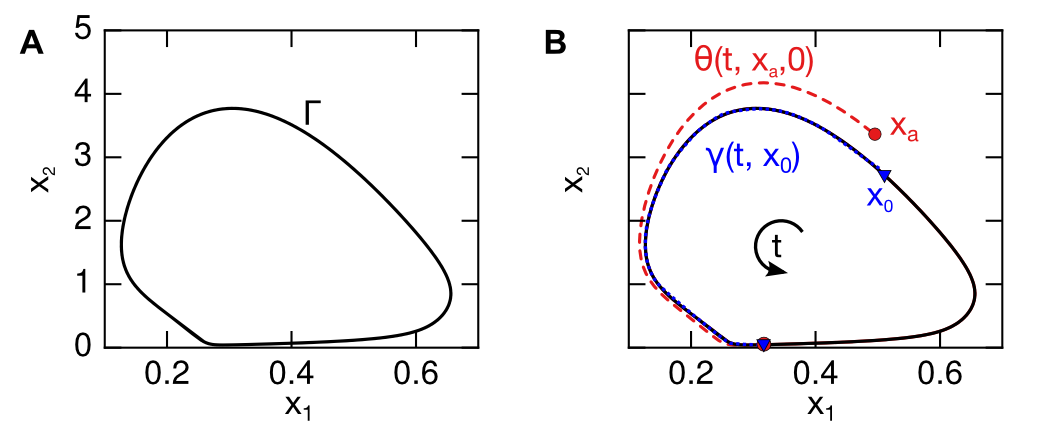
\includegraphics[width=8.4cm]{chap6/figures/figure_-1.png}    % The printed column
\end{center}
\caption{Schematic of limit cycle dynamics for arbitrary states $x_1$ and $x_2$.
		(\textbf{A}) The limit cycle $\Gamma$ in state space.
		(\textbf{B}) Schematic of trajectories $\gamma$ and $\theta$. These points may be assigned identical phases ($\phi_a = \phi_0$), as the trajectories originating at these points converge asymptotically.
        \label{fig:-1}  }                               % Size the figures                               % accordingly.
\end{figure}

This chapter is concerned with dynamics of the phase of oscillation, and so we first map every unique point on the limit cycle $x_0\in\Gamma$ to a unique scalar phase $\phi_0\in\mathbb{S}^1=[0,2\pi)$.
Let $\Phi : \Gamma \to \mathbb{S}^1$ denote the corresponding map relating $x_0$ to oscillator phase $\phi_0 = \Phi(x_0)$.

Let $\gamma(t, x_0)$ denote the solution of system \eqref{eq:odes6} with initial condition $x(0) = x_0\in\Gamma$.
Thus a time-dependent phase variable
\begin{equation}
    \phi(t) = \Phi[\gamma(t,x_0)]
\end{equation}
may be established.
Considering that the unperturbed oscillator traverses the limit cycle at the constant rate $\omega$, the system phase evolves in time according to:
\begin{equation}
    \label{eq:phasevar1}
    \phi(t) = \omega\,t+\phi_0 \; \mod\, 2\pi.
\end{equation}


The application of an exogenous input (such as a control action) will divert the state of an oscillatory system away from the limit cycle $\Gamma$.
In order to ascertain the phase shift incurred by such an input, we must assign a phase to points that are not on the limit cycle $\Gamma$, but that are exponentially attracted to $\Gamma$.
This can be done by assigning them the phase of the trajectory to which they ultimately converge.
The trajectory denoted $\theta(t,x_a,u)$ is the time evolution of point $x_a\notin\Gamma$, with dynamics given by \eqref{eq:odes6} and control input $u$.
For the zero-input case ($u=0$), the state $x_a$ may be assigned the phase of the initial condition of the trajectory $\gamma(t, x_0)$ to which the trajectory $\theta(t,x_a,0)$ ultimately converges.
The asymptotic phase of $x_a$, denoted $\phi_a$, is equal to the phase $\phi_0$ of point $x_0\in\Gamma$, subject to
\begin{equation}
    0 = \lim_{t\to\infty}||\theta(t, x_a,0) - \gamma(t, x_0)||.
\end{equation}
This relationship yields the asymptotic phase map $\phi_a = \mathit{\Phi}(x_a)$.
The asymptotic phase map may be used to formulate a time-dependent asymptotic phase variable for the zero-input case
\begin{equation}
    \varphi(t,0) = \mathit{\Phi}[\theta(t,x_a,0)]
\end{equation}
for the zero-input case.
The trajectories $\gamma$ and $\theta$ with identical phase, and their asymptotic convergence, are shown schematically in Fig.~\ref{fig:-1}B.



This formulation yields phase dynamics identical to the case for $\phi$, with particular solutions of the form $\varphi(t,0) = \omega\,t+\phi_0$ with initial phase $\phi_0$.
The following subsection described how the concept of an asymptotic phase variable can be extended for the more challenging and useful case of non-zero control input $u$.

\subsection*{Infinitesimal parametric phase response curves and the phase-reduced model}


For an oscillator in the neighborhood of $\Gamma$, the phase dynamics resulting from a control input may be derived by the chain rule:% in a similar fashion as in \cite{Efimov2009}: they use this term neighborhood
\begin{equation}\label{eq:firstord}
    \frac{d\varphi(t,u)}{dt} = \omega + \frac{\partial}{\partial t}\frac{\partial\mathit{\Phi}[\gamma(t,x_0)]}{\partial u}u(t)
\end{equation}
which yields a first-order approximation of phase dynamics for a nonzero control input.

Pharmaceutical manipulations of the clock are generally considered to be mediated by temporary changes in one or more parameter values (e.g. increased degradation of a protein, or decreased transcriptional rate) \cite{Hirota2012a, Kim2013}.
% justification of use of parametric PRC from here
Input $u(t)$ is incorporated into the ODE model as a time-dependent modification of parameters $p$
\begin{equation}
    p(t) = p_0+u(t).
\end{equation}
Substituting this into \eqref{eq:firstord} yields
\begin{equation}
    \label{eq:phiipprc}
    \frac{d\varphi}{dt} = \omega + \frac{\partial}{\partial t}\frac{\partial\mathit{\Phi}[\gamma(t,x_0)]}{\partial p}u(t),
\end{equation}
where $\frac{\partial}{\partial t}\frac{\partial\mathit{\Phi}[\gamma]}{\partial p}$ is the infinitesimal parametric PRC (ipPRC) for the oscillator on the limit cycle \cite{Taylor2008a}.
The formulation \eqref{eq:phiipprc} is valid up to the first-order approximation in both duration and magnitude of the control, and is referred to as the \textit{phase-reduced model}.
The one-dimensional phase equation is therefore given by:
\begin{equation}\label{eq:osc}
    \frac{d\varphi}{dt} = \omega + B(t, \varphi)\cdot u(t),
\end{equation}
where $B(t,\varphi)$ is the ipPRC and $u(t)$ is the parametric perturbation.


\begin{asm}\label{asm:1}
    The ipPRC $B(\cdot)$ is fully known and dependent only on the asymptotic phase $\varphi(t)$.
\end{asm}
The ipPRC can be calculated numerically from mechanistic models of the clock for a known control input as above, or alternately could be characterized experimentally \cite{Taylor2008a,Johnson1999}.
A prior method of formulating asymptotic phase dynamics assumed short pulses of control inputs that relax completely to the limit cycle after each pulse \cite{Efimov2009}, and thus the phase sensitivity on the limit cycle may be used.
Assumption \ref{asm:1}, rather, implies that the phase response dynamics are constant along isochrons (state-space regions of constant phase).
This assumption is violated as the oscillator becomes more distant from its limit cycle, or closer to the fixed point at the center of the limit cycle.
Identifying violations of this assumption may be studied in the future, and in these cases, the model should be simulated in full.
This assumption has been used in prior studies as well \cite{Qiao2017, Julius2017}.
Our assumption yields a few practical advantages when implementing pharmaceutical inputs.
Short pulses are less able to evoke significant phase shifts, as the realized phase shift is determined by integration of the ipPRC.
Thus, the ipPRC must be of extreme magnitude to yield appreciable shifts for short pulses.
Pharmaceutical inputs to the clock are not likely to have the extremely rapid pharmacokinetics needed to be approximated as short pulses.

\begin{asm}
    The ipPRC map is continuous on $[0, 2\pi]$ and has exactly two zero crosses in that interval; the derivatives of the ipPRC at the zero crosses have opposite sign.\label{asm:2}
\end{asm}

This PRC form is readily found in the literature, and for stimuli of a finite duration is commonly referred to as a type 1 phase response \cite{Winfree2001, Johnson1999}.
Methods for calculation of the ipPRC using limit-cycle oscillator models are described elsewhere \cite{Taylor2008a}.
The other phase response observed (solely) for finite-duration stimuli, a type 0 phase response, contains a discontinuity.
This form is associated with strong and extended stimulus or multiple stimuli over several days, and therefore does not correspond to the ipPRC \cite{Winfree2001, Johnson1999, Kronauer1999}.
Furthermore, a type 0 phase response may be generated from an ipPRC that conforms to Assumption \ref{asm:2} by applying a long-duration stimulus.



\subsection*{The phase resetting problem and optimal phase resetting via Pontryagin's maximum principle \label{ssec:optimal}}

The phase-resetting problem involves tracking a reference oscillator with phase given by $\varphi_r(t)\in[0,2\pi)$, with the oscillator $\varphi(t,u)$ which obeys \eqref{eq:osc}, and with control input bounded by $u\in[u_{\rm min}, u_{\rm max}]$.
The phase of the reference oscillator is given by:
\[
    \varphi_r(t) = \omega_r\,t+\varphi_r(0) \; \mod\,2\pi.
\]

\begin{asm}
    The reference angular velocity is identical to the angular velocity of the oscillator, that is, $\omega\equiv\omega_r$.
\end{asm}
\begin{asm}
    The oscillator is not perturbed by exogenous inputs other than control actions.
\end{asm}
    Through these assumptions we seek to achieve a phase shifts rather than entrain to a dynamic phase angle or an environment that also phase shifts oscillation.
    The more complicated case, in which small differences in the human circadian period (see \cite{Czeisler1999}) and dynamic light input are accounted for, may be approached by future studies.
This simple case of achieving a static phase shift more simply yields optimal control policies that are sufficient to provide understanding for feedback controller design.

The phase difference between the reference oscillator and the oscillator under control is:
\begin{equation*}
    \chi(t) = \varphi(t)-\varphi_r(t) \; \mod2\pi.
\end{equation*}
The total desired phase shift is such that $\chi(t_f) = 0$, and therefore
\begin{equation*}
\Delta\phi_f = -\chi(0)\,\mod2\pi.
\end{equation*}

In an ideal case where pharmaceutical inputs can be continuously dosed, one can derive an optimal control trajectory for entrainment via Pontryagin's Maximum/Minimum Principle \cite{Kirk2012pontryagin}.
The optimal control problem may be formulated with state dynamics
\begin{align}\label{eq:ode}
        \dot\varphi &= \omega + B(\varphi)\cdot u(t)\\
        \nonumber\varphi(0) &= \phi_0,
\end{align}
and cost functional
\begin{equation}\label{eq:j}
    J[u(t)] = \int_0^{t_f} 1\, dt.
\end{equation}
This yields a free-time fixed-endpoint problem, which can be solved using standard optimal control approaches \cite{Kirk2012pontryagin, Qiao2017}.
The Hamiltonian
\begin{equation}\label{eq:hamiltonian}
        H(\varphi,\lambda,u) = (\omega+B(\varphi)\cdot u)\cdot\lambda +1
    \end{equation}
    is formulated with $\lambda$ is the dynamic costate with terminal condition $\lambda(t_f)=0$.
Using Pontryagin's Maximum Principle with constrained control inputs in the range $[u_{\rm min}, u_{\rm max}]$ we can write
    \begin{align*}
        \max_{u} H(\varphi,\lambda,u)&= \max_{u_{\min}\leq u\leq u_{\max}}\{(\omega+B(\varphi)\cdot u)\cdot\lambda +1\}\\
        \nonumber &= \omega\cdot\lambda + 1+ \max_{u_{\min}\leq u\leq u_{\max}}\{B(\varphi)\cdot u \cdot\lambda\}
    \end{align*}
which yields the optimal ``bang-bang'' control policy
    \begin{equation}
    u^\star(t) = \begin{cases}u_{\max} &\mbox{if } B(\varphi)\cdot\lambda >0 \\
        u_{\min} & \mbox{if }B(\varphi)\cdot\lambda \leq0 \end{cases}.
    \end{equation}
    Here, the terminal condition of the costate, $\lambda(t_f)=0$, forces the costate to be either positive or negative for any given initial condition for all time, and so for a specific initial condition the control input depends exclusively on the sign of $B(\varphi)$, c.f.\ \cite{Qiao2017}.



This implies that the oscillator should be shifted in only either the negative or positive direction toward its final phase shift, but not both.
For an oscillator with desired phase shift $\Delta\phi_f$ and initial phase $\phi_0$, the optimal control input $u^\star$ is one of two admissible trajectories: either that for achieving the positive phase shift
\begin{equation}
    u^\star_{+}(t) = \begin{cases}u_{\max} &\mbox{if } B(\varphi) >0 \\
        u_{\min} & \mbox{if } B(\varphi) \leq0 \end{cases}
\end{equation}
or the negative phase shift
\begin{equation}
    u^\star_{-}(t) = \begin{cases}u_{\min} &\mbox{if } B(\varphi) \geq0 \\
        u_{\max} & \mbox{if } B(\varphi) <0 \end{cases}.
\end{equation}
Which of these two trajectories is optimal depends upon which reaches $\Delta\phi_f$ more rapidly, where $\Delta\phi$ accumulates according to
\begin{equation}\label{eq:delphi}
    \Delta\phi = \int_0^{t}B(\varphi(t'))\cdot u(t')dt'\; \mod\,2\pi.
\end{equation}
A decision boundary between advances and delays is denoted $\Delta\phi_b$ (i.e., $\Delta\phi_f > \Delta\phi_b$ indicates that delays are preferable, and $\Delta\phi_f < \Delta\phi_b$ indicates that advances are preferable).
Correspondingly, that boundary for the continuous time optimal control is denoted $\Delta\phi^\star_b$.
Thus, the two admissible trajectories may be calculated and compared to determine optimality.

This concept is illustrated for small-molecule pharmaceutical KL001 input in Fig.~\ref{fig:0} and Fig.~\ref{fig:optimal}.
First, we selected the model from \cite{Hirota2012a,StJohn2014a} to capture circadian oscillator dynamics because it was created to identify the effect of the small-molecule KL001 on the mammalian oscillator.
Model states and reactions are shown schematically in Fig.~\ref{fig:0}A, and the equations and parameters comprising this model are shown in Table~\ref{tab:stjohnmodel}.
The control input was included as a reduction of parameter $v_\text{dCn}$, as identified in \cite{StJohn2014a}, leading to the ipPRC of Fig.~\ref{fig:0}B.
Next, the optimal control law was applied in Fig.~\ref{fig:optimal}.
\begin{table}[p]
    \caption{Model equations and parameters for the core clock feedback loop from \cite{StJohn2014b}, continued on the following page.}
  \label{tab:stjohnmodel}
  \vspace{2mm}
  \centering
\begin{tabular}{l l l}\hline
	State Variable & Symbol & Conservation Equation\\
	\hline\\
	\textit{Per} mRNA & \textbf{p} & $\frac{d\mathrm{\bf p}}{dt}     = \frac{v_{\text{txn,{\bf p}}}}{k_{\text{txn,{\bf p}}} + \left(\text{\bf C1N} + \text{\bf C2N} \right)^3} - \frac{v_{\text{deg,{\bf p}}} \;\text{\bf p} }{k_{\text{deg,{\bf p}}} +\text{\bf p} }$
	\\[0.4cm]
	\textit{Cry1} mRNA & \textbf{c1} & $\frac{d\text{\bf c1}}{dt}    = \frac{v_{\text{txn,{\bf c1}}}}{k_{\text{txn,{\bf c}}} + \left(\text{\bf C1N} + \text{\bf C2N} \right)^3} - \frac{v_{\text{deg,{\bf c1}}} \;\text{\bf c1} }{k_{\text{deg,{\bf c}}} +\text{\bf c1} }
$ 
	\\[0.4cm]
	\textit{Cry2} mRNA & \textbf{c2} & $    \frac{d\text{\bf c2}}{dt}   = \frac{v_{\text{txn,{\bf c2}}}}{k_{\text{txn,{\bf c}}} + \left(\text{\bf C1N} + \text{\bf C2N} \right)^3} - \frac{v_{\text{deg,{\bf c2}}} \;\text{\bf c2} }{k_{\text{deg,{\bf c}}} +\text{\bf c2} }
$ 
	\\[0.4cm]
	\textit{Per} Protein & \textbf{PER} & \splitcell{
		$\frac{d\text{\bf P}}{dt}   = k_\text{tln,{\bf p}} \;\text{\bf p}  - \frac{v_{\text{deg,{\bf P}}} \;\text{\bf P} }{k_{\text{deg,{\bf P}}} +\text{\bf P} } - v_{\text{a,{\bf CP}}} \;\text{\bf P}  \;\text{\bf C1}  + v_{\text{d,{\bf CP}}} \;\text{\bf C1N}$\\[0.3cm] $ \qquad- v_{\text{a,{\bf CP}}} \;\text{\bf P}  \;\text{\bf C2}  + v_{\text{d,{\bf CP}}} \; \text{\bf C2N}
	$ }
	\\[0.4cm]
	\textit{Cry1} Protein & \textbf{C1} & $\frac{d\text{\bf C1}}{dt}  =\text{\bf c1}  - \frac{v_{\text{deg,{\bf C1}}} \;\text{\bf C1} }{k_{\text{deg,{\bf C}}} +\text{\bf C1} } - v_{\text{a,{\bf CP}}} \;\text{\bf P}  \;\text{\bf C1}  + v_{\text{d,{\bf CP}}} \;\text{\bf C1N}
$ 
	\\[0.4cm]
	\textit{Cry2} Protein & \textbf{C2} & $\frac{d\text{\bf C2}}{dt}    =\text{\bf c2} - \frac{ (v_{\text{deg,{\bf C2}}}-u(t)) \;\text{\bf C2} }{k_{\text{deg,{\bf C}}} +\text{\bf C2} } - v_{\text{a,{\bf CP}}} \;\text{\bf P}  \;\text{\bf C2}  + v_{\text{d,{\bf CP}}} \; \text{\bf C2N}
$ 
	\\[0.4cm]
    CRY1-PER Dimer & \textbf{C1N} & $\frac{d\text{\bf C1N}}{dt}   = - \frac{ (v_{\text{dCn}-u(t))} \;\text{\bf C1N} }{k_{\text{deg,{\bf CP}}} +\text{\bf C1N}  + \text{\bf C2N} } + v_{\text{a,{\bf CP}}} \;\text{\bf P}  \;\text{\bf C1} - v_{\text{d,{\bf CP}}} \;\text{\bf C1N}
$ 
	\\[0.4cm]
	CRY2-PER Dimer & \textbf{C2N} & $\frac{d\text{\bf C2N }}{dt}  = - \frac{ \left(v_{\text{dCn}} \; m_{\text{\bf C2N}}\right) \; \text{\bf C2N} }{k_{\text{deg,{\bf CP}}} + \text{\bf C2N}  +\text{\bf C1N} } + v_{\text{a,{\bf CP}}} \;\text{\bf P}  \;\text{\bf C2} - v_{\text{d,{\bf CP}}} \; \text{\bf C2N}
$\\[0.4cm] 
\hline
\end{tabular}
\end{table}

\clearpage
\begin{table}
\contcaption{(Continued.)}
    \centering
\begin{tabular}{cllrr} \hline
    & Parameter                 & Description                       & Value \\ \hline\\
    1  & $v_{\text{txn,{\bf p}}}$  & {\it Per} Transcription rate      & 0.195        \\
    2  & $v_{\text{txn,{\bf c1}}}$ & {\it Cry1} Transcription rate     & 0.131        \\
    3  & $v_{\text{txn,{\bf c2}}}$ & {\it Cry1} Transcription rate     & 0.114        \\
    4  & $k_{\text{txn,{\bf p}}}$  & {\it Per} Repression constant     & 0.425        \\
    5  & $k_{\text{txn,{\bf c}}}$  & {\it Cry1/2} Repression constant  & 0.259        \\
    6  & $v_{\text{deg,{\bf p}}}$  & {\it Per} Max degradation rate    & 0.326        \\
    7  & $v_{\text{deg,{\bf c1}}}$ & {\it Cry1} Max degradation rate   & 0.676        \\
    8  & $v_{\text{deg,{\bf c2}}}$ & {\it Cry2} Max degradation rate   & 0.608        \\
    9  & $k_{\text{deg,{\bf p}}}$  & {\it Per} Degradation constant    & 0.011        \\
    10 & $k_{\text{deg,{\bf c}}}$  & {\it Cry1/2} Degradation constant & 1.149        \\
    11 & $v_{\text{deg,{\bf P}}}$  & Max PERc degradation rate         & 2.970        \\
    12 & $k_{\text{deg,{\bf P}}}$  & PERc degradation constant         & 0.034        \\
    13 & $v_{\text{deg,{\bf C1}}}$ & Max CRY1c degradation rate        & 1.523        \\
    14 & $v_{\text{deg,{\bf C2}}}$ & Max CRY2c degradation rate        & 1.686        \\
    15 & $k_{\text{deg,{\bf C}}}$  & CRYc degradation constant         & 2.017        \\
    16 & $v_{\text{dCn}}$ & CRYn degradation rate             & 0.101        \\
    17 & $m_{\text{\bf C2N}}$      & CRY2n degradation multiplier      & 3.318        \\
    18 & $k_{\text{deg,{\bf CP}}}$ & CRYn degradation constant         & 0.053        \\
    19 & $v_{\text{a,{\bf CP}}}$   & CRYn association rate             & 0.041        \\
    20 & $v_{\text{d,{\bf CP}}}$   & CRYn dissociation rate            & 0.002        \\
    21 & $k_{\text{tln,{\bf p}}}$  & PER translation rate              & 3.000        \\ \hline
    \hline
  \end{tabular}
\end{table}


\begin{figure}[p]
    \begin{center}
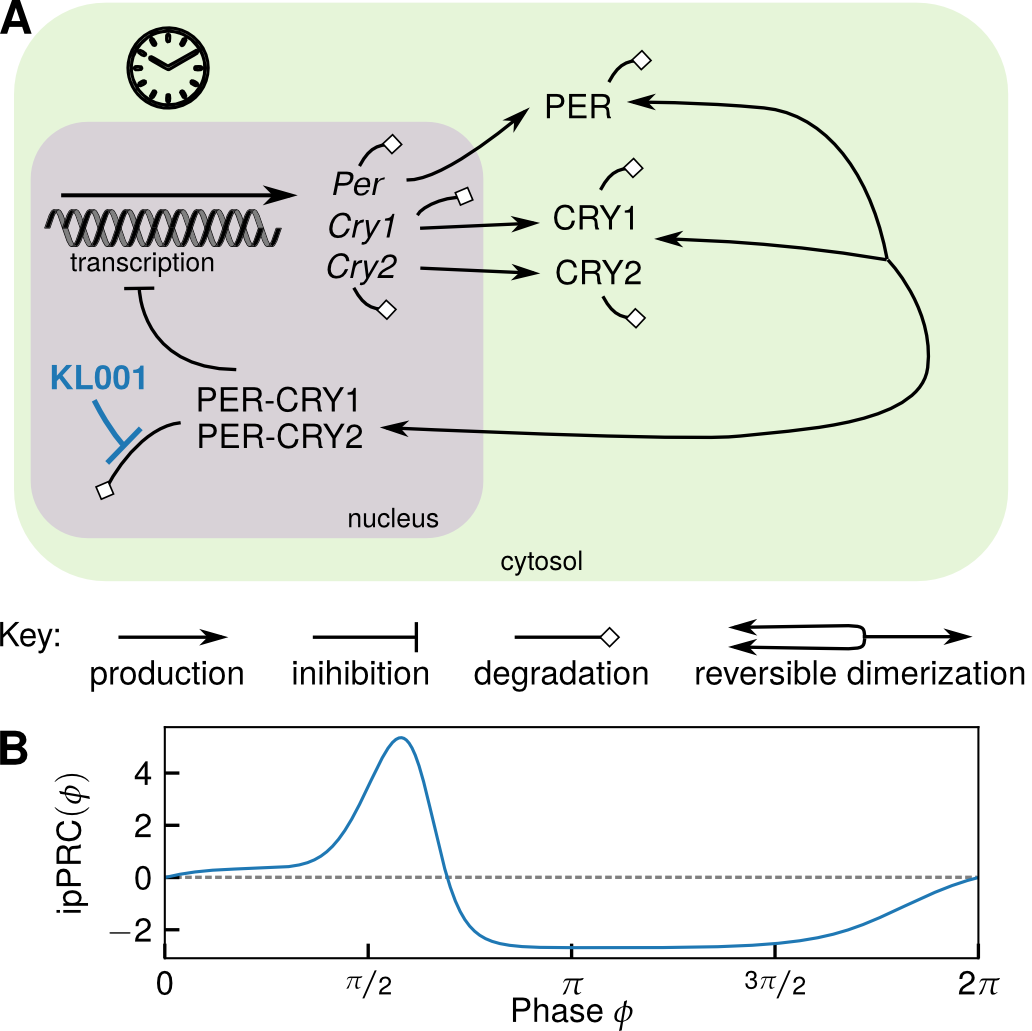
\includegraphics[width=8.4cm]{chap6/figures/figure_0.png}    % The printed column
\end{center}
\caption{Schematic of the core circadian gene regulatory network and effect of small molecule KL001.
		(\textbf{A}) The core circadian negative feedback loop. KL001 stabilizes nuclear CRY by reducing its degradation rate, as shown in blue. All reactions in the figure are explicitly incorporated in the clock model used \cite{StJohn2014b}, and the full equations are provided in Table~\ref{tab:stjohnmodel}.
		(\textbf{B}) Infinitesimal parametric phase response curve (ipPRC) for KL001-mediated stabilization of nuclear CRYs as calculated from the model.}  % width is 8.4 cm.
\label{fig:0}                                 % Size the figures                               % accordingly.
\end{figure}


\begin{figure}[p]
    \begin{center}
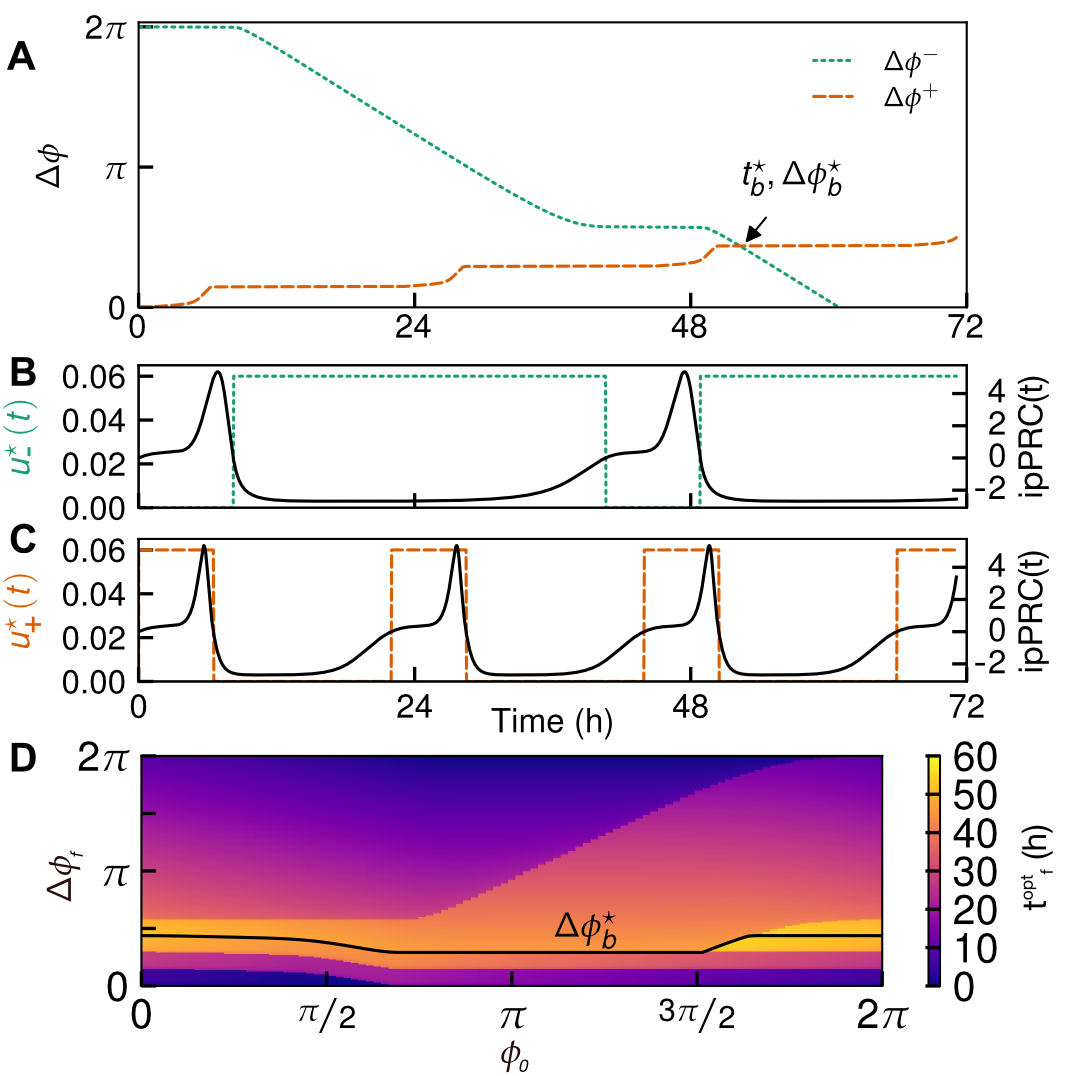
\includegraphics[width=8.4cm]{chap6/figures/figure_1.png}    % The printed column
\end{center}
\caption{\label{fig:optimal}Optimal control of the circadian clock by use of the ipPRC shown in Fig.~\ref{fig:0}B. (\textbf{A}) Maximal phase advances $\Delta\phi^\star_+(t)$ and delays $\Delta\phi^\star_-(t)$ for the ipPRC, with $\phi_0 = 0$ and $u_{\max} = 0.06$, $u_{\min} = 0.00$. The respective maximal phase shifts meet at time $t^\star_b$ and phase shift $\Delta\phi^\star_b$ as marked on the graph. All phase shifts may be achieved in time less than or equal to $t^\star_b$.
  Note that $t^{\rm opt}_f(0, \Delta\phi_f)$ can be found on this plot by seeking the minimum time at which the oscillator crosses the desired $\Delta\phi_f$ (for example, $t^{\rm opt}_f(0, 3\pi/2) \approx 20$ h, and is achieved by a phase delay).
  (\textbf{B,C}) Plot of optimal inputs $u^\star_-(t)$ and $u^\star_+(t)$, respectively, for the phase delay and advance shown in A.
  (\textbf{D}) Heatmap of optimal time to reset the clock $t^{\rm{opt}}_f$ as a function of initial phase as desired shift. Note that $\Delta\phi^\star_b$, the boundary between advances and delays, is dependent on $\phi_0$.}  % width is 8.4 cm.
% Size the figures                              % accordingly.
\end{figure}

We may visualize the two admissible trajectories as two oscillators $\varphi^{+}(t)$ and $\varphi^{-}(t)$ receiving control inputs $u^\star_{+}(t)$ and $u^\star_{-}(t)$, respectively, causing the accumulation of phase shifts $\Delta\phi^{+}(t)$ and $\Delta\phi^{-}(t)$ moving in opposite directions around the circle of all phase shifts $\Delta\phi\in[0,2\pi)$ starting at $\Delta\phi=0$.
The time $t^\star_b$ at which these oscillators meet therefore achieves any phase shift on $[0,2\pi)$.
    This time may be found for any initial phase $\varphi(0)=\phi_0$ by solving the coupled equations \eqref{eq:osc} and \eqref{eq:delphi} for inputs $u^\star_{+}(t)$ and $u^\star_{-}(t)$, with the terminal condition of $\Delta\phi^{+}(t^\star)=\Delta\phi^{-}(t^\star)$.

Thus, $\Delta\phi^\star_b(\phi_0)$ is defined as the phase shift at which $\varphi^{-}(t)$ and $\varphi^{+}(t)$ meet.
The maximum time to achieve \textit{any} phase shift starting from $\phi_0$ is given by $t^\star_b(\phi_0)$, and $\Delta\phi^\star_b(\phi_0)$ (depicted as a solid black line in Fig.~\ref{fig:optimal}D) yields the boundary between where a positive shift and negative shift are optimal to reach a desired $\Delta\phi_f$ from phase $\phi_0$.
The optimal control input for a given $\phi_0$ and $\Delta\phi_f$ is therefore defined as:
\begin{equation}\label{eq:policy}
    u^\star(t) = \begin{cases}u^\star_+(t) &\mbox{if } \Delta\phi_f < \Delta\phi^\star_b(\phi_0) \\
       u^\star_-(t) &\mbox{if } \Delta\phi_f \geq \Delta\phi^\star_b(\phi_0) \end{cases}.
\end{equation}
Therefore the optimal shift time $t^{\rm opt}_f(\phi_0,\Delta\phi_f)$ may be calculated by applying this continuous time optimal control until $\Delta\phi=\Delta\phi_f$.
One can formally write $t^\star_b$ as
\begin{equation}
    t^\star_b(\phi_0) = \sup_{\Delta\phi_f} t^{\rm opt}_f(\phi_0,\Delta\phi_f).
\end{equation}

\begin{rmk}
A bang-bang optimal control policy for light entrainment was shown previously in \cite{Serkh2014} and \cite{Zhang2016}.
Applying these solutions, however, necessitated either a line search or a search for switching times due to the nonlinear temporal relationship between light input and driving force on the oscillator.
Because pharmaceutical control of the clock can be parameterized directly within the limit cycle model, this formulation provides a simple way to compute the theoretical optimal phase resetting policy.
Therefore, this provides a means for determining the relative efficacy of any applied control policy.
\end{rmk}
%One drawback of this approach is its treatment of the organism as a single-oscillator system.
%In actuality, each cell within an organism contains an autonomous oscillator, and population synchrony in addition to mean phase should be considered in future studies of circadian resetting \revi{maybe cite emerging appl chapter?}.
%Furthermore, this approach ignores the pharmacokinetics of any drug applied in a physically realizable system.
%This formulation may be used, then, to compare the efficiency of a drug with its theroetical optimal properties.

\section{Closing the loop: designing a PRC-based nonlinear MPC\label{sec:fb}}



\subsection*{Motivation}
Model predictive control is generally implemented by solving a finite-horizon optimal control problem at discrete sampling times, that is, for $t=0,\tau,2\tau,\cdots$ where $\tau$ is the sampling time.
This section will demonstrate that time discretization causes a loss of optimal control in regions where the step includes a zero cross of the ipPRC, as the input cannot be adjusted during the step and the continuous-time optimal control policy will be violated (visualized in Fig. \ref{fig:zerocross}).
Additionally, care must be taken to ensure that a controller selects the optimal direction of phase shifting (e.g., 8h advance vs. 16h delay) when only observing a finite portion of the future PRC.
For the continuous time optimal control, that boundary is known to be $\Delta\phi^\star_b$, however, this is unlikely to be the correct boundary for the sampled-time case.
Further, there is no guarantee that this boundary will appear from simply solving the finite-horizon optimal control.

\begin{figure}[p]
    \begin{center}
    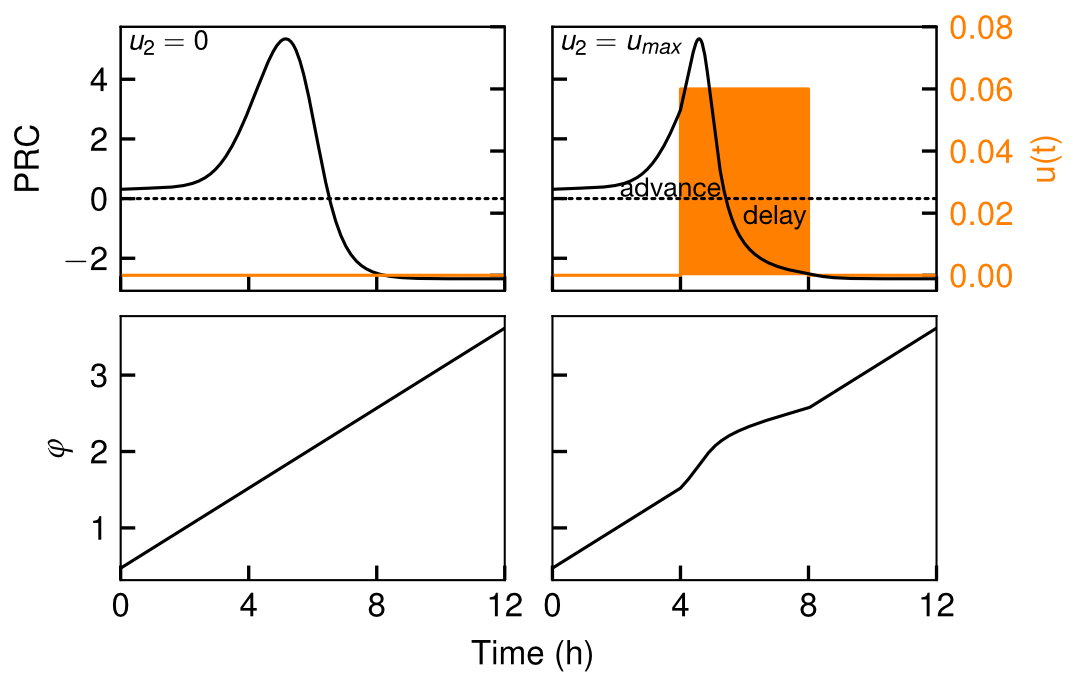
\includegraphics[width=8.4cm]{chap6/figures/figure_3.png}
\end{center}
    \caption{\label{fig:zerocross} Error in applying the optimal control policy occurs at the zero-crosses of the ipPRC. For a sampling time of 4 h, the zero-cross occurs in the second step $t_1<t^0<t_2$, and so $u_2$ will necessarily violate the continuous-time optimal control law. For the cases shown here, $\Delta\phi_2(u_{\rm max}) = \Delta\phi_2(u_{\rm min}) = 0$, and the resulting phase is identical due to cancellation of the advance by the delay. Finally, it is noteworthy that this single pathological step consumes most of the positive lobe of the PRC, suggesting that $\tau=4$~h is a poor choice for sampling time if phase advances are desirable.}
\end{figure}

This section explores how the formulation of the finite-horizon optimal control problem for MPC affects our ability to control the clock.
For example, consider an ipPRC with a small positive lobe.
A large sampling time in this case may result in a controller unable to access the positive ipPRC region due to the surrounding negative region being included in each step, and the inadvertent delays canceling the desired advance.
This would force such a controller to use phase delays to achieve even small positive phase shifts.

It is therefore useful to compare the performance of a controller with piecewise constant control and uniformly spaced steps in sampling and switching time (the \textit{sampling-time control}) to the continuous-time optimal control case to identify where inefficiency accumulates.
This technique can be used to find a balance between high performance and the computational cost and physical impracticality of frequently updating the algorithm via measurement of physiological phase markers.

Additionally, the controller design will inform the suitability of a specific pharmaceutical for use.
For example, a drug with a small positive ipPRC lobe will not be an appropriate choice for achieving large phase advances if an alternative drug with a larger positive ipPRC lobe exists.
Alternately, the drug with the larger positive ipPRC lobe may be unsuitable if its pharmacokinetics are slow, such that sampling times must be very long to allow drug clearance between adjusting the dose.

\subsection*{Exploiting the ipPRC to choose MPC sampling time}


Consider the more practical scenario of implementing control inputs parameterized as piecewise constant signals with equispaced time intervals between the knots of the control parameterization trajectory.
This is commonly done when solving and applying MPC in continuous-time.
The control input is defined as constant across time steps of uniform duration in a finite horizon, as commonly done for MPC:
\begin{equation}\label{eq:sampled_control_law}
    u(t) = u_i \; \mathrm{for} \; t\in[t_{i-1},t_{i}),
\end{equation}
where $t_i$ are the discrete sampling times, with $i=1,\cdots, N_p$ where $N_p$ is the number of steps in the prediction horizon (and control horizon, in this chapter).
Then, $u_i\in[u_{\rm min},u_{\rm max}]$ is a scalar constant, and $\tau = t_{i}-t_{i-1}$ is the sampling time for the controller.

The error incurred due to piecewise constant control actions at discrete sampling times is quantified via two metrics, the first of which is described in the following definition.
\begin{defn}
	\label{defn:res_phase_err}
The \textbf{residual phase error} ($E^{\phi}_\tau$) is the phase error remaining at sampling time $t_k$, the first sampling time for which the continuous-time optimal control would have first completed the reset.
\end{defn}

Recall that $t^{\rm{opt}}_f$ is the time at which $\chi(t)=0$ under the optimal control and so
\begin{equation} k = \arg\min\limits_{i\in\mathbb{N}} i\;\; \text{subject to:}\;\; t_i\geq t_f^{\rm opt}.
\end{equation}
Based on Definition~\ref{defn:res_phase_err}, the residual phase error is given by
\begin{equation}
    E^{\phi}_\tau = \chi(t_k).
\end{equation}
First, we provide bounds on these two metrics and demonstrate that these bounds are solely dependent on the sampling time $\tau$ and the ipPRC specific to the pharmaceutical being used.


\begin{thm}[Bounding of $E^\phi_\tau$]
    Suppose Assumptions 1-4 hold. Let $n_{\rm cyc}$ be the number of $2\pi$ cycles required to achieve the continuous time optimal control resetting using the optimal control policy~\eqref{eq:policy}. The residual phase error incurred by the sampled-time control~\eqref{eq:sampled_control_law} satisfies
\begin{equation*}
    E^{\phi}_\tau \leq (n_{\rm cyc}+1)(E^{0,-}_\tau +E^{0,+}_\tau + E^s)
\end{equation*}
where $E^{0,-}_\tau$, $E^{0,+}_\tau$, and $E^s$ are the errors incurred at the negative zero cross, the positive zero cross, and a correction for phase advance cases, respectively.
\end{thm}
    \begin{proof}
    Note that the sampling-time control is able to identically track the continuous-time optimal control except where consecutive sampling times occur on either side of a zero-cross of the ipPRC.

    By Assumption~\ref{asm:2}, the ipPRC has two zero-crosses in each $[0,2\pi)$ cycle and so this occurs at most twice per cycle. A zero cross occurs at $t=t^0$ (where $t_{i-1} < t^0 < t_i$).
The maximal loss of phase advance or delay is incurred if the switching times are positioned such that the shift incurred over that time step $\Delta\phi_i(u_i) = 0$, where
\begin{equation}
    \Delta\phi_i(u_i) = \int_{t_{i-1}}^{t_i} B(\varphi(t'))\cdot u_i\,dt',
\end{equation}
which must be solved numerically with \eqref{eq:osc} to provide $\varphi(t')$.
Based on the arguments made in the previous section using Pontryagin's principle, we know that $u_i$ is either $u_{\rm max}$ or $u_{\rm min}$.

The maximal loss in phase shift is of equal magnitude in the positive and negative directions because competing advances and delays of identical magnitudes cancel.
The maximal error incurred at a given zero-cross is
\begin{equation}
    %\begin{split}
    E^0_\tau = \max\limits_{t_{i-1}, u} \,\left| \int_{t_{i-1}}^{t^0} B(\varphi(t'))\cdot u \,dt'\right|%\\
%    &\int_{t_{i-1}}^{t^0} B(\varphi(t'))\cdot u_{\rm min} dt' \big),
%\end{split}
\end{equation}
and the error for the positive or negative zero-cross is denoted $E^{0,+}_\tau$ and $E^{0,-}_\tau$, respectively.
The maximal phase error incurred for each cycle is the sum of the maximal error from each zero-cross, all other steps are identical to the continuous-time optimal control.
A demonstration of the phase-shift cancellation by competing advances and delays is shown in Fig.~\ref{fig:zerocross}.

For phase advances, additional error is incurred by phase advances accumulating less due to the zero crosses, thus, the oscillator phase will reach the next positive ipPRC lobe later than it would if it could achieve the full phase advance.
The additional error accumulated is equal to the maximal shift that could be achieved in the extra time that it takes to reach the positive lobe.
The time lost per cycle for phase advances is:
\begin{equation}
    t_E = \frac{T}{2\pi}\cdot(E^{0,+}_\tau + E^{0,-}_\tau)
\end{equation}
which results in an additional residual phase error per cycle of
\begin{equation}
    E^s = \begin{cases}
        \max\limits_{0\leq t\leq T} \int_t^{t+t_E}B(\varphi(t'))\,dt'&\mbox{if } \Delta\phi_f < \Delta\phi_b\\
        0 & \mbox{if }\Delta\phi_f \geq \Delta\phi_b  \end{cases},
\end{equation}
where $\Delta\phi_b$ is the decision boundary between phase advances and delays.
In the case of phase delays, this quantity is 0, since the oscillator phase will reach the next negative lobe more rapidly due to achieving less phase delay.
Thus, we can bound the residual time phase error
\begin{equation}\label{eq:ephi}
    E^{\phi}_\tau \leq (n_{\rm cyc}(\Delta\phi_f, \phi_0)+1)(E^{0,-}_\tau +E^{0,+}_\tau + E^s)
\end{equation}
for a given $\tau$, which concludes the proof.
\end{proof}


The bound $E^{\phi}_\tau$ may be thought of as the maximal value of $\chi(t_k)$ for optimal control with sampling time $\tau$.
\begin{rmk}
At first glance, it may seem that this bound is loose for the case of arbitrarily large $n_{\rm cyc}$, the number of cycles to achieve any reset is bounded by the finite scalar
\begin{equation*}
n_{\rm cyc}^{\max} = \max\limits_{\Delta\phi_f, \phi_0} n_{\rm cyc}(\Delta\phi_f, \phi_0)
\end{equation*}
the maximum number of number of cycles to achieve any continuous time optimal reset.
Applying this value in \eqref{eq:ephi}, we may bound the residual time phase error for any sampling-time optimal reset.
\end{rmk}

Fig.~\ref{fig:stepsize1} shows how the residual phase error bounds evolve over time for phase advances or delays, $\phi_0=0$, and $\tau=2$~h.
This corresponds to the actual residual phase error incurred, by numerically calculating the optimal control.
Although the error bound increased identically for each cycle, the actual residual phase error varies each cycle, depending upon how each zero-cross aligns with the sampling times.

\begin{figure}[p]
    \begin{center}
    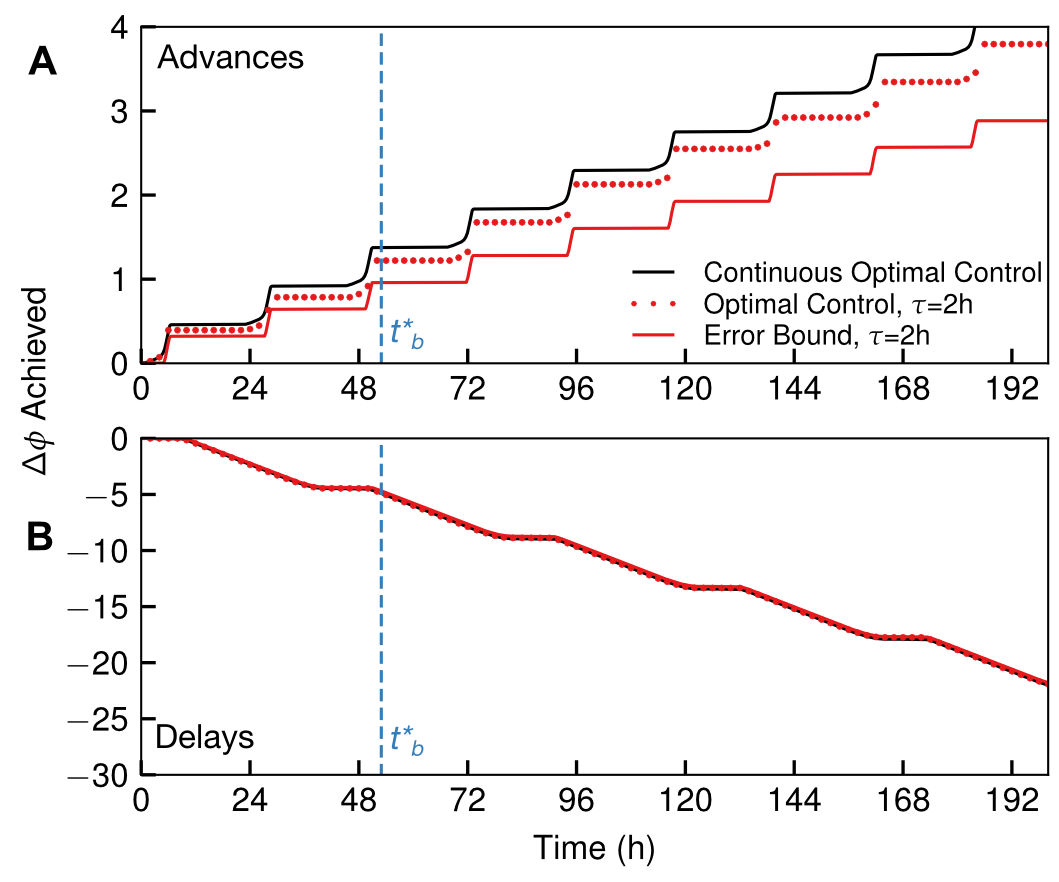
\includegraphics[width=3.5in]{chap6/figures/figure_4.png}
\end{center}
      \caption{\label{fig:stepsize1} The bound on residual phase error (red line) and the actual residual phase error (red dots) plotted as a function of time, in comparison to the continuous-time optimal control (black line), for $\tau=2$ h and $\phi_0=0$. Phase advances (\textbf{A}) and delays (\textbf{B}) are shown explicitly. The bound deviates further from the optimal control at each completed cycle, however, only the shifts that occur before $t^\star_b$ (dashed line) are attempted under the optimal control policy. Additionally, the error is more severe for phase advances, due to the relatively smaller positive region of the ipPRC, and the proximity of that positive region to a large negative region. For panel B, these lines are nearly on top of one another. The numerically-calculated optimal control for $\tau=2$ h indeed obeys the bounds derived in Theorem 1 from the continuous time optimal control.}
\end{figure}


Fig.~\ref{fig:stepsize2}A-B demonstrates this bound for KL001 under $\tau = 1,2,4$ h, for $\phi_0 = 0$.
The number of cycles to achieve each reset for phase advances or delays $\Delta\phi_f\in[-2\pi,2\pi]$ (to explicitly show advances and delays) and $\phi_0=0$ under the continuous-time optimal control for KL001 is shown in Fig.~\ref{fig:stepsize2}A.
The region of this plot that corresponds to the phase resetting directions selected by the continuous-time optimal control (advances for $\Delta\phi_f < \Delta\phi_b^\star$, delays for $\Delta\phi_f \geq \Delta\phi_b^\star$) are denoted between the dashed lines.
Notably, the number of cycles to achieve phase advances accumulates more rapidly due to the smaller positive lobe of the PRC, and as such, error will incur more quickly in phase advance regions.
Fig.~\ref{fig:stepsize2}B shows the bounds on the residual phase error for $\tau = 1,2,4$ h, and the actual residual phase error incurred for numerically calculating the optimal control for each shift and sampling time.
As observed, the calculated residual phase errors fall within the computed bounds.

\begin{figure}[p]
    \begin{center}
	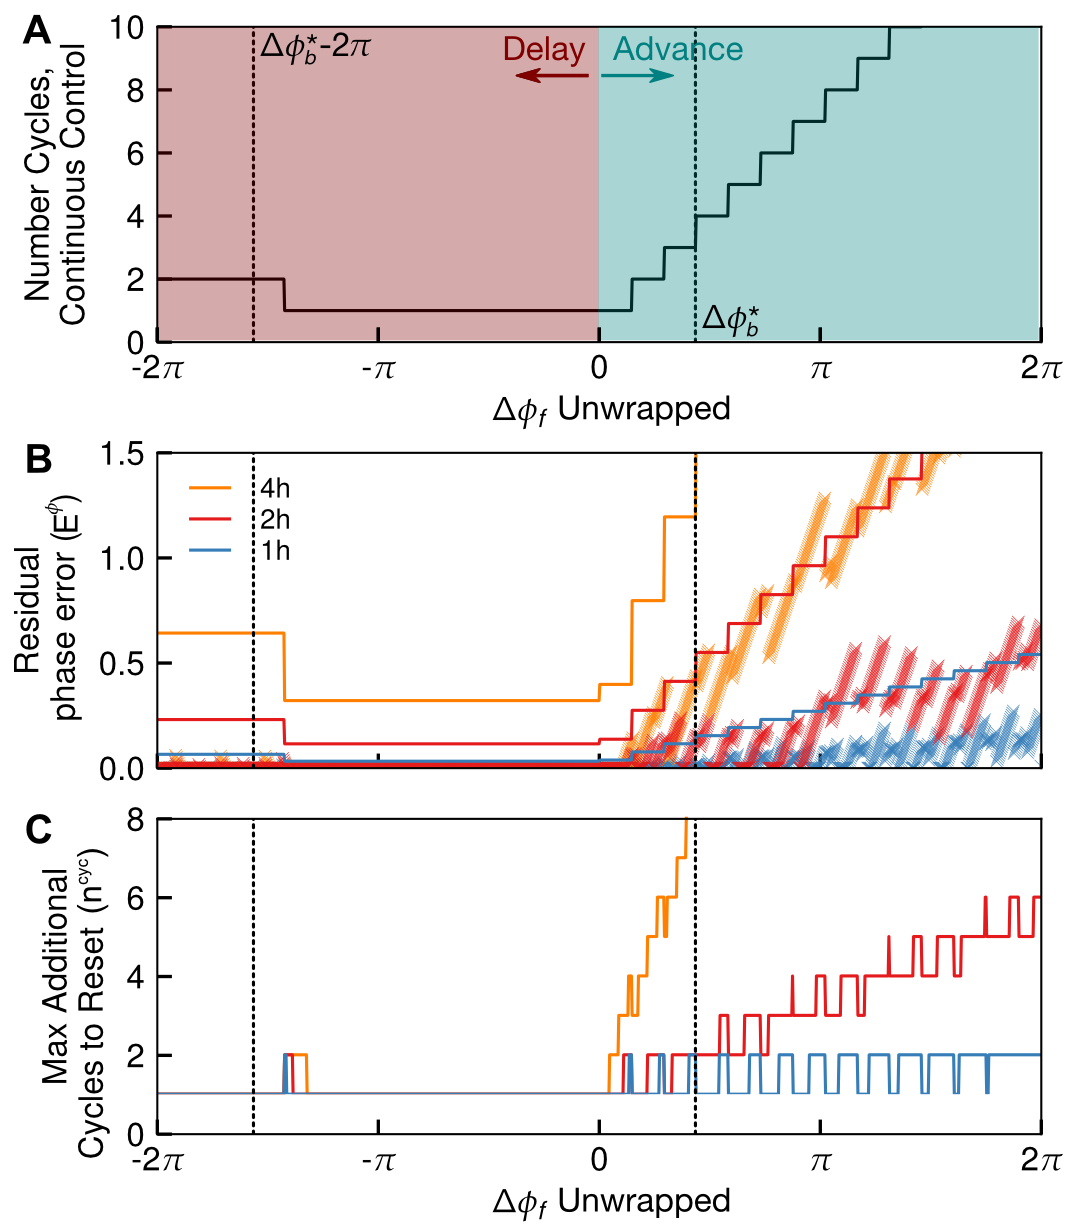
\includegraphics[width=8.4cm]{chap6/figures/figure_5.png}
\end{center}
	\caption{\label{fig:stepsize2} Sampling time $\tau$ affects circadian phase resetting for optimal control with evenly-spaced switching times, a common feature of feedback control and MPC. (\textbf{A}) Plot of number of cycles required to achieve each phase advance or delay under continuous-time optimal control. Errors due to switching timing occurs where the ipPRC crosses 0, and thus is residual phase error is a function of the number of cycles required for continuous-time optimal control. (\textbf{B}) A bound on $E_\tau^\phi$, the distance to the final phase that will remain at $t = t_f^{\rm opt}$ under optimal control with a constant sampling time is derived from the continuous optimal control trajectory. Here, the derived bound is shown as a line, and the numerically calculated optimal control solutions are shown as x markers for each $\tau$. The residual phase error in each case indeed obeys the theoretical bounds. (\textbf{C}) A bound on $n_{\rm cyc}^{\rm add}$ is also derived. For this example, 1~h and 2~h shifts yield similar residual phase error and allow a complete reset in at most two additional cycles, under $\Delta\phi^b=\Delta\phi^\star$. Thus, either is a reasonable choice for sampling time, though a 2~h sampling time will reduce the cost of sampling by half. Alternately, if this drug were used only to achieve phase delays, a 4~h sampling rate would be similarly suitable.}
\end{figure}

In addition to the residual phase error, it is useful to determine how much additional time it would take to reach a complete reset.
Effectively, we aim to find $t^{\rm add}$ for $\chi(t^{\rm opt}_f+t^{\rm add}) = 0$.
Finding or bounding $t_e$ is complicated, as finding it necessitates knowledge of the entire optimal control trajectory for each $\phi_0$ and $\Delta\phi_f$. An abstraction is used to gather data about this additional time, described in the following definition.
\begin{defn}
The \textbf{number of additional cycles to complete reset} ($n^{\rm add}_\tau\in\mathbb{N}$) is a positive scalar that enforces the constraint
\[
\chi(t_f+n_{\rm cyc}^{\rm add}T^{+,-})=0,
\]
where $T^{+,-}$ is the accelerated/decelerated period of the oscillator induced by a phase advance/delay, respectively.
\end{defn}
\begin{rmk}
Clearly, $T^{+} < T < T^{-}$, and by virtue of being on a limit cycle yields
\begin{equation*}
\lim_{t\to\infty}[x(t,p,u_+) - x(t-T^{+},p,u_+)]=0
\end{equation*}
and
\begin{equation*}
\lim_{t\to\infty}[x(t,p,u_{-}) - x(t-T^{-},p,u_{-})]=0
\end{equation*}
where $u_+$ and $u_-$ are control inputs resulting in phase advances or delays, respectively.
\end{rmk}

The following upper bound is proposed on the number of additional cycles to complete reset.

\begin{thm}[Bounding of $n_{\rm cyc}^{\rm add}$]
    Let $\Delta\phi^-_{g,\tau}$ and $\Delta\phi^+_{g,\tau}$ be the maximum phase delay and advance that is guaranteed to be achievable in a cycle of $2\pi$, respectively. Recall that $\Delta\phi_b$ is the decision boundary between phase advances or delays.
    The number of additional cycles to correct for the residual phase error incurred by the sampled-time control~\eqref{eq:sampled_control_law} is bounded above by
    \begin{equation}\label{eq:thm2}
        n_{\rm cyc}^{\rm add} \leq \begin{cases}\floor{E^{\phi}_\tau / \Delta\phi^+_{g,\tau}}+1 &\mbox{if } \Delta\phi_f \leq\Delta\phi_b \\
            \floor{E^{\phi}_\tau/\Delta\phi^-_{g,\tau}}+1 & \mbox{if }\Delta\phi_f \geq\Delta\phi_b \end{cases},
\end{equation}
where $\floor{\cdot}$ denotes the floor function.
\begin{proof}

Let $\Delta\phi^+_{g,\tau}$ denote the phase advance that are guaranteed to be achievable in a single cycle.
This is more simply thought of as the maximum total phase advance or delay achievable in a cycle minus the worst-case zero-cross error.
For advances, the maximum phase advance achieved in a cycle is achieved by the continuous time optimal control policy for advances:
\begin{equation}
    \Delta\phi^+_{\rm cyc} = \int_0^{T^+} B(\varphi(t'))\cdot u^\star_{-}(t')dt'.
\end{equation}
The phase shift that is guaranteed to be achievable for each cycle for a step size of $\tau$ is therefore
\begin{equation}
    \Delta\phi^+_{g,\tau} = \Delta\phi^+_{\rm cyc} - E^{0,+}_\tau - E^{0,-}_\tau,
\end{equation}
and an equivalent method can be used to calculate $\Delta\phi^-_{g,\tau}$.

The bound may be calculated by dividing the remaining error $E^{\phi}_\tau$ by the advance or delay that is guaranteed to be achieved each cycle for a sampling time of $\tau$. This implies~\eqref{eq:thm2}.
\end{proof}
\end{thm}



This bound is plotted for the use of KL001 and $\tau = 1,2,4$ h in Fig.~\ref{fig:stepsize2}C.
For sampling times of 1 or 2 h, the residual phase error may corrected in 1-2 cycles, with the vast majority of cases needing only an additional cycle.
Furthermore, because this method assumes the worst possible alignment of the control switching times for every cycle, it is unlikely that the full two additional cycles will be needed.
Alternately, the 4 h sampling time potentially results in many additional cycles needed to achieve a complete reset.
This is because, as shown in Fig.~\ref{fig:zerocross}, a 4 h step could be aligned such that nearly the entire phase advance region of the ipPRC is lost.
Correspondingly, $\Delta\phi^+_{g,\tau}$ is small in value.
Thus, we may conclude that a sampling time of 2 h is approximately as effective as 1 h, and provides a 50\% reduction in computational and sampling costs over 1 h sampling times, given our assumptions.
Our controller designed in Section~\ref{sec:ex} therefore uses $\tau=2$ h.
However, if a controller was designed to only produce phase delays, a 4 h sampling time is sufficiently near to the optimal control.
This metric is therefore useful in designing controllers for a given problem and potential pharmaceutical given its ipPRC.

For these plots, dashed lines bound the phase shifts that are performed by the continuous-time optimal control to achieve complete coverage of phase shifts from 0 to $2\pi$.
This implicitly assumes that the direction of optimal phase shifting is known for our choice of $\tau$, and is identical to the continuous time optimal control bound $\Delta\phi^\star$.
The following subsection addresses the choice of resetting direction (given $\Delta\phi^\star$ for the continuous optimal case).

While numerical calculation of the infinite-horizon optimal control may seem advantageous, the optimizations involved are costly, as the selection of each step affects the region of the ipPRC available in the ensuing steps.
Rather, we propose to formulate the MPC problem using the bounds derived from the optimal control as guidelines, and perform phase shifts by repeatedly solving the finite-horizon optimal control.
It must be emphasized that because the bound we have derived is for the maximum residual phase error incurred at each zero-cross, a controller need not solve the infinite-time optimal sampling time control to be governed by the bound.
Solving a finite-horizon optimal control problem is sufficient for these bounds on accumulated error to apply.


\subsection*{On MPC formulation and the selection of a prediction and control horizon}



MPC involves repeatedly solving a finite horizon optimal control problem.
For the continuous-time optimal control (in Section~\ref{ssec:optimal}) the direction of phase shifting was determined by calculation of the equal-time phase shift boundary $\Delta\phi^\star$.
For MPC, whether the oscillator should advance or delay is implicitly solved in the finite horizon optimization.
This subsection demonstrates via simulations that the finite-horizon optimal control in MPC is dependent on the number of steps.
Ultimately, we propose a multi-staged optimization for solving the finite-horizon optimal control.

The MPC problem is formulated in a similar fashion as \cite{Abel2016b}, where the prediction and control horizons are set to be identical.
The prediction horizon consists of $N_p$ steps with sampling time $\tau$.
For an oscillator at $t=t_k$ this yields:
\begin{eqnarray}
U&\triangleq& \begin{bmatrix} u(t_k+\tau) & \cdots & u\left(t_k+N_p\tau\right)
\end{bmatrix}^\top
\end{eqnarray}
as the knots of the control trajectory defined at each of the $N_p$ steps.
Eqn.~\eqref{eq:osc} is used as the MPC predictor, which estimates the oscillator phase at the end of each of $\ell\in[1,\cdots,N_p]$ steps.
The predictor formulation of \eqref{eq:osc} is
\begin{equation}\label{eq:discretephase6}
    \hat\varphi(t_i+\ell\tau) = \varphi(t_i) + \omega\tau -\sum_{k=1}^{\ell} \int_{t_{i}+(k-1)\tau}^{t_{i}+k\tau} B(\varphi)\cdot u_k\, dt.
\end{equation}
Here, $i$ is the index of the applied control steps, and $k$ is the index of the predictor.
The predicted phase error $\hat \chi(t)$ is defined as the magnitude of the phase difference between the predicted phase $\hat \varphi$ and the environmental phase:
\begin{equation}
    \label{eq:predictor}
        \hat{\chi}(t) \triangleq \hat\varphi(t)-\varphi_r(t) \,\,\,\mod\,2\pi.
\end{equation}
Driving phase error to precisely zero is numerically unstable, so we ignore phase error below a constant $\delta_\phi$:
\begin{equation}
    g_{\phi}(t)  \triangleq \begin{cases}
            0 & \text{if}\ |\hat\chi(t)|<\delta_\phi\\
            \hat\chi(t) & \text{otherwise}
        \end{cases}
 \end{equation}
so that numerical imprecisions do not result in controller action.
Thus, the finite-horizon optimal control problem at each time $t_i$ may be solved for the optimal trajectory $u^\star_{\rm MPC}$:
\begin{eqnarray}
    \nonumber  u^\star_{\rm MPC} &= \arg\min\limits_{U} \;\sum_{\ell=1}^{N_p} w^\phi g^2_{\phi}(t_i+\ell\tau) + w^u u_\ell^2\\
        \label{eq:mpcoptim6} &\text{subject to:}\\
        \nonumber &\text{Eqn. \eqref{eq:predictor}}\\
        \nonumber  &u_{\min} \le u_{\ell}\le u_{\max},
    \end{eqnarray}
for all $\ell=1, \cdots,N_p$, where $w^\phi$ and $w^u$ are positive weighting scalars evaluated at the end of the time step and start of the time step, respectively, as phase error is calculated after the control is applied for that step.
After identifying the optimal piecewise control trajectory $u^\star$, the initial step $u^\star_1$ is applied to the system (in this case the full 8-state ODE model) for $t \in (t_i, t_i+\tau]$ as is standard in model predictive control.

For the ensuing simulations, a sampling time of $\tau = 2$ h was used, as described in the prior section.
Additionally, weights $w^\phi = 10$ and $w^u = 1$, so that no control is delivered for marginal gains in phase shifting, and $\delta_\phi=0.1$ as in \cite{Abel2017a}.

Simulations demonstrate that the optimization step in the MPC is susceptible to errors induced by choosing the slower direction to achieve a phase reset.
The example in Fig.~\ref{fig:horizon} shows how the finite horizon optimal control $u^\star_{\rm MPC}$ calculated for $\Delta\phi_f = \pi$, $\phi_0=0$ varies with $N_p$.
For short prediction horizons, the controller applies a phase advance, because more of the positive ipPRC lobe is immediately visible to the predictor, suggesting that this will achieve most rapid reset.
By extending the prediction horizon to $N_p = 10$ (20 h), more of the negative lobe of the ipPRC is available, and so the controller waits for this region before applying input, consistent with the infinite-time optimal control for $\tau = 2$ h.
In some cases, performing the optimization in this manner could result in an ``indecisive'' controller that changes directions during the phase shifting, causing excessive lags to reset.

\begin{figure*}[p]
    \begin{center}
    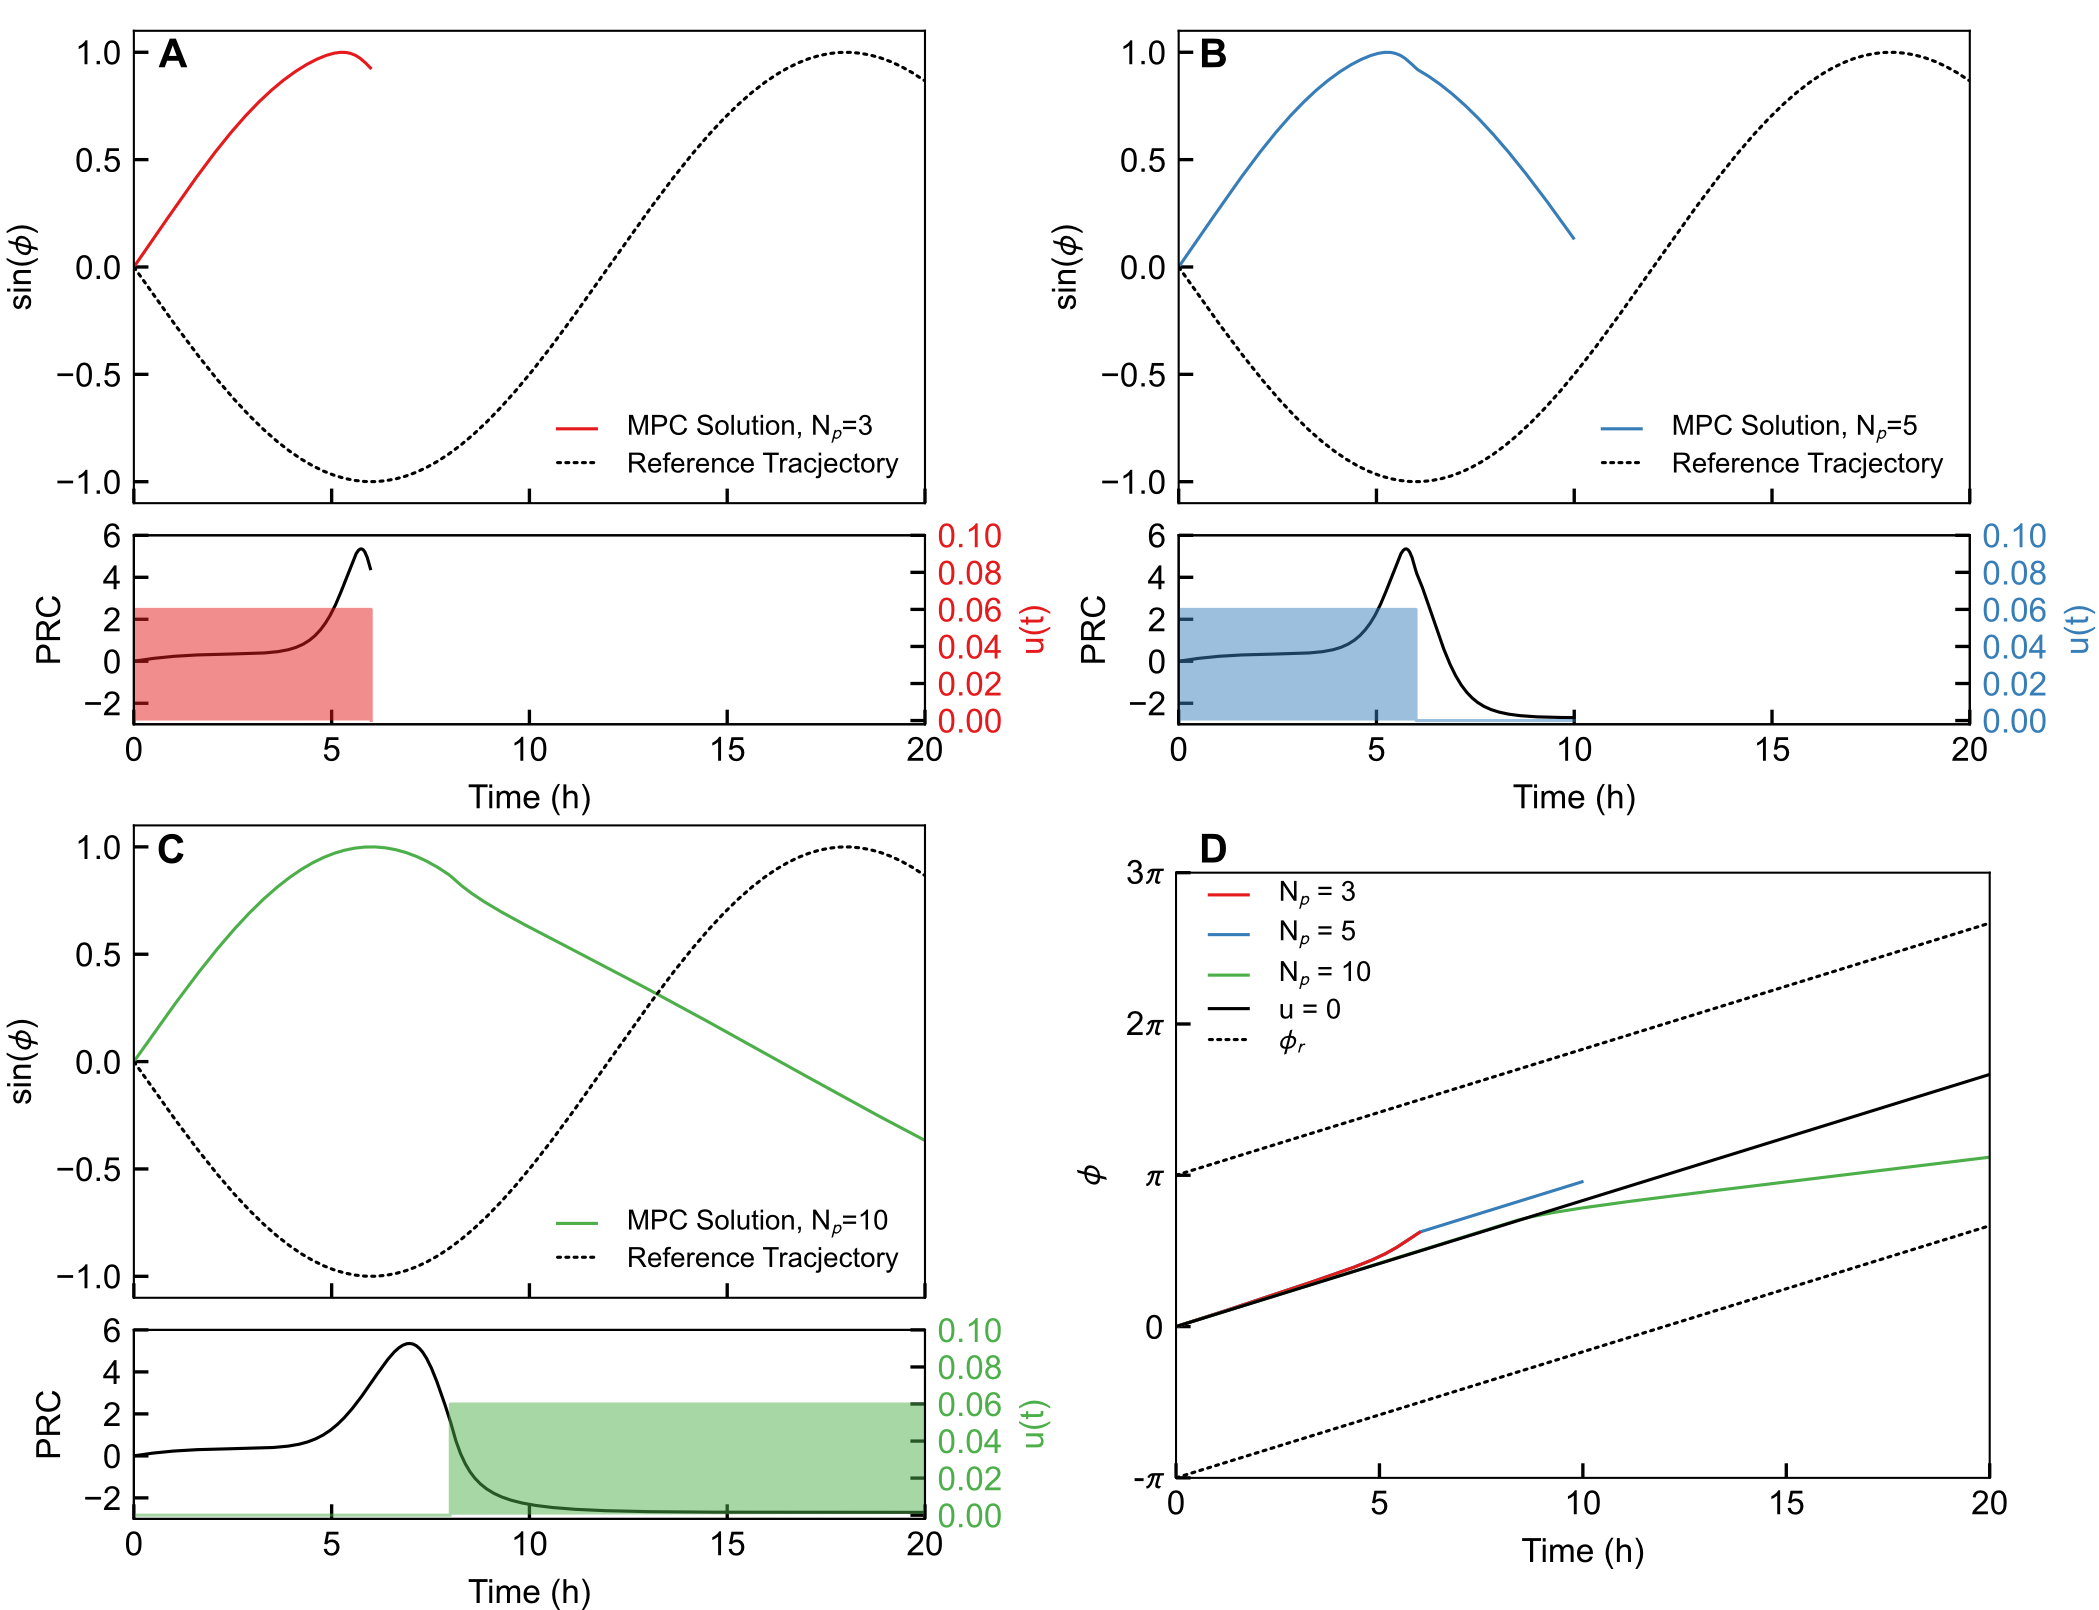
\includegraphics[width=\textwidth]{chap6/figures/figure_6.png}
\end{center}
      \caption{\label{fig:horizon}
      Changes in the prediction horizon affect the finite-horizon optimal control trajectory based on the observable PRC. This is demonstrated by computing the first finite-horizon optimal control trajectory and varying that horizon. (\textbf{A-C}) Finite-horizon optimal control trajectories for $N_p=3,\,4,\text{ and } 5$, respectively. In all cases, $\tau=2$h, $\Delta\phi_f=\pi$, and $\phi_0=0$. Note that not only do the finite horizon optimal controls computed by the MPC differ, they seek to achieve the same shift by either advances (A,B) or delays (C). The infinite-horizon optimal control is achieved via delays ($\Delta\phi_f > \Delta\phi^\star$), and so A or B would lead to excessively-long resetting by either selecting advances to achieve the shift, or first selecting advances then later choosing delays.
      (\textbf{D}) This result is visualized by plotting the phase progression for each MPC case and for the 0-input case. Phase advances evidently yield slower progress toward the reference phase, and thus short prediction horizons choose ineffectively. This complication in MPC problem formulation may be circumvented by providing the controller with the optimal resetting direction \textit{a priori}.
  }
\end{figure*}



One solution to the problem of inconsistent finite-horizon optimal control policies is to extend the prediction horizon such that it always observes the entirety of the reset, to guarantee that the finite-horizon optimal control calculated during MPC is equal to the infinite-horizon optimal control, that is: $u^\star_{\rm MPC} = u^\star_{\rm \tau}$.
However, this leads to excessive computational costs, especially for small sampling times.
Furthermore, the optimization formulation itself poses challenges.
Minimizing the time to complete the reset is challenging, as there is no gradient along which to move unless the reset is completed during the prediction horizon, leading to cases with an infinite cost.
Minimizing phase error at each step may be suboptimal as well: the fastest reset achievable may involve temporarily increasing $\chi(t)$ for cases where $\Delta\phi_f<\pi$ and $\Delta\phi_f>\Delta\phi_\tau^\star$.

An alternate approach, which is employed in the following section, is to use a two-stage optimization, where the direction of the reset (advance or delay) is chosen first using bound $\Delta\phi^b$.
Furthermore, we propose using  $\Delta\phi^b = \Delta\phi^\star$, as this will ensure that the bounds on residual phase error and additional cycles to reset hold, as derived in the prior section, and thus provide guarantees on controller performance in the absence of plant-model mismatch or noise.
One further important consideration is that a controller with $N_p = 1$ will be unable to avoid accumulating error at the zero-crosses, whereas a controller with a larger $N_p$ provides flexibility to adjust the control inputs preceding a zero-cross to minimize the accumulated error.
For this reason, the design parameters were set to $N_p = 5$ and $\Delta\phi^b= \Delta\phi^\star$ for our controller.
We note, however, that the derived bounds hold even for $N_p=1$.

\section{In silico application of designed MPC controller for phase resetting\label{sec:ex}}
To demonstrate the efficacy of this control approach, this section presents two control scenarios in our \textit{in silico} circadian simulator (shown schematically in Fig.~\ref{fig:scheme}).
The controller used has $\tau=2$h, $N_p = 5$, and $\Delta\phi^b = \Delta\phi^\star$, as prescribed by the design considerations in the prior sections.



The first scenario (Fig.~\ref{fig:mpc_demo}) is an example of extreme jet lag, in which the environment undergoes a 5 h phase advance, followed three days later by a phase delay of 11 h.
This is the equivalent of a flight from Boston to London, then London to Honolulu.
Here, the controller first waits for a positive region of the PRC rather than immediately attempting a delay, as $\Delta\phi_f < \Delta\phi^b$.
Thus, it completes this phase advance in approximately 30 h.
The 11 h delay occurs during a region where $B(\varphi)<0$, and thus control input is provided immediately.
This shift is completed in a total of two continuous doses, in approximately 36 h.
Without a control approach, light input alone achieves a shift of 2-3h per day at most, thus, this represents a significant speed up in phase resetting.
If light is delivered under optimal control, these shifts are predicted to take several days \cite{Serkh2014}, thus demonstrating the potential for improvement by a pharmaceutical input.

The second scenario (Fig.~\ref{fig:mpc_demo2}) involves the delivery of KL001 to align an individual working on a rotating shift pattern, from \cite{Vetter2015}.
Here, the time on the x-axis is local time, and the phase of the oscillator is initialized for an individual entrained to a normal light-dark cycle.
In this protocol the individual works two days of morning shift, followed by two days of evening shift, followed by two days of night shift (work shifts denoted by gray boxes.
This perpetually phase-delaying schedule is easily tracked by KL001 input, as KL001 more easily achieves phase delays.
Notably, by taking one large dose after the conclusion of each pair of shifts, the individual rapidly shifts to the new work phase.
Each shift worked in this protocol occurs while the individual is exactly phase-aligned with their work environment.
This scenario exclusively involves phase delays, and so under the analysis of Section~\ref{sec:fb} a larger sampling time of $\tau = 4$ h (or possibly even larger) would be similarly effective.

Importantly, the possibly competing effects of light was neglected in these scenarios.
This could be achieved simply by restricting light input during the phase-shifting steps, or treating light as a complementary control input, using an approach such as \cite{Julius2017}.
This is a possible topic for future study.

\begin{figure}[p!]
	\centering
    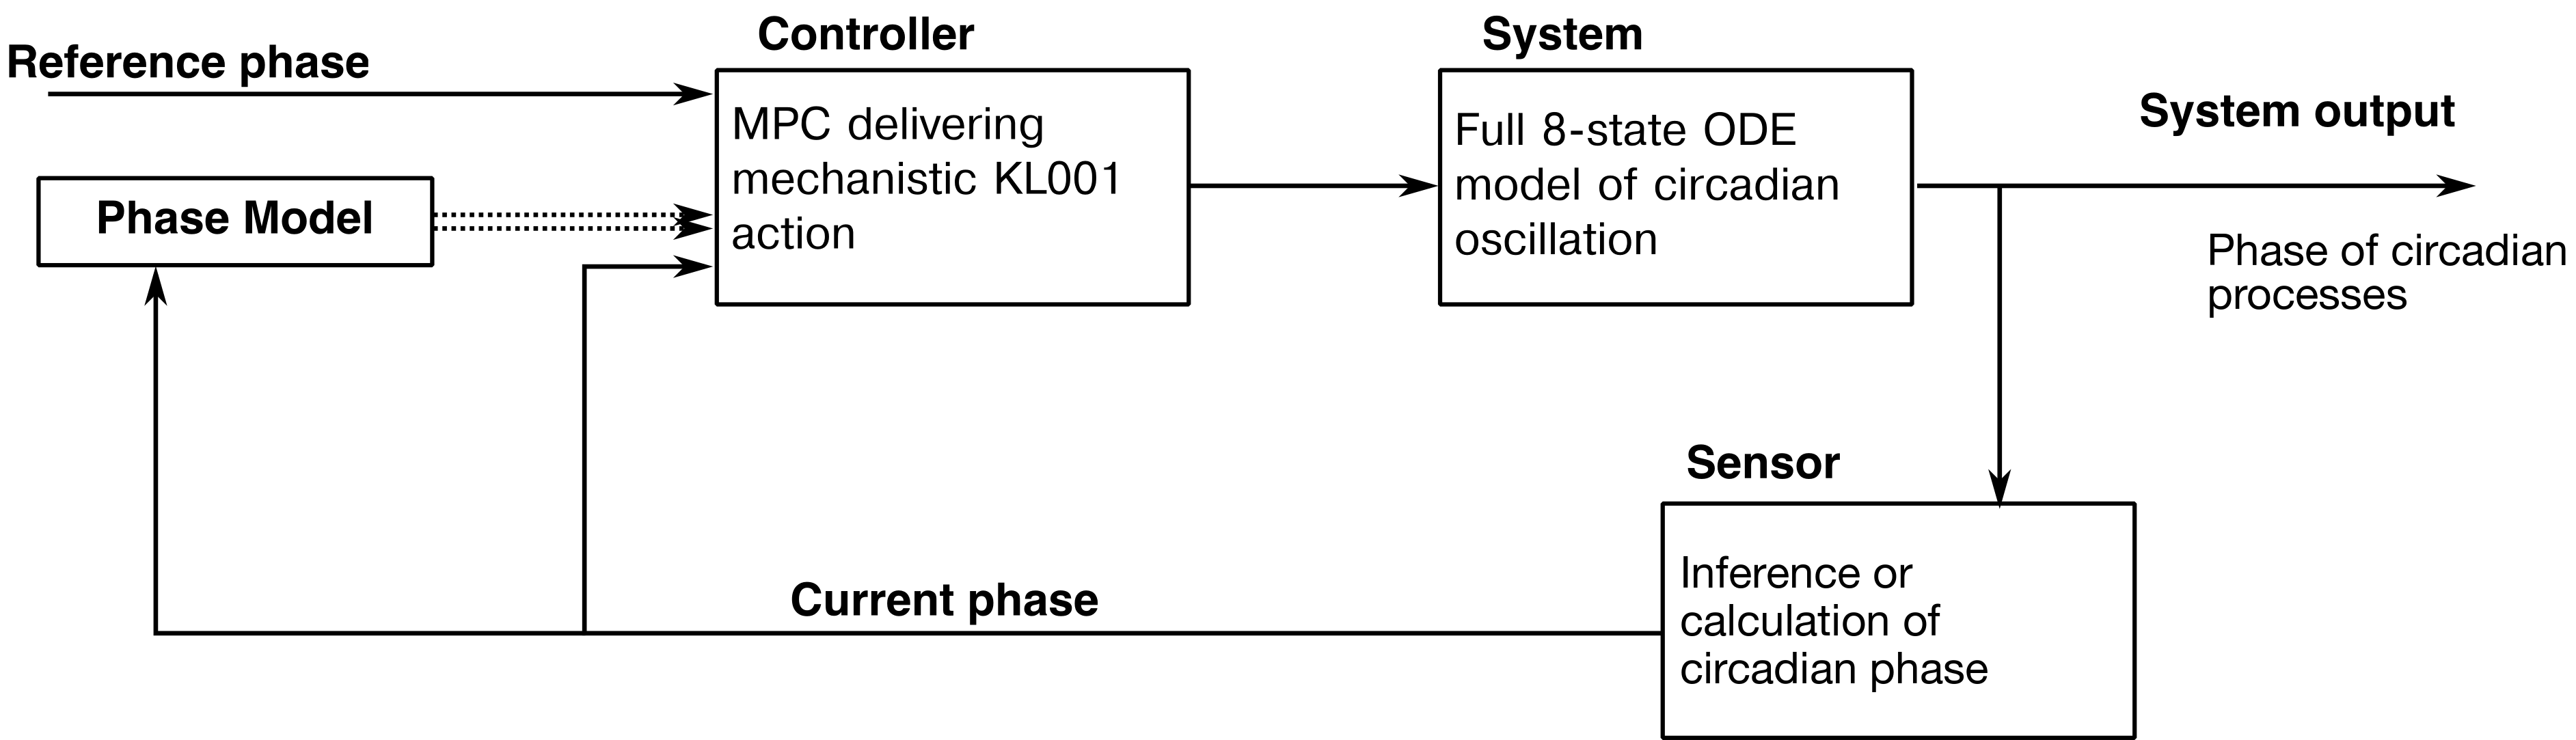
\includegraphics[width=7in]{chap6/figures/figure_2.png}
    \caption{\label{fig:scheme} \textit{In-silico} scheme for MPC of circadian rhythms. In experimental or clinical application, the human, organism, or cell culture would replace the 8-state ODE model (Table~\ref{tab:stjohnmodel}) as the system under control.}
\end{figure}

\clearpage
\begin{figure*}[p]
    \begin{center}
    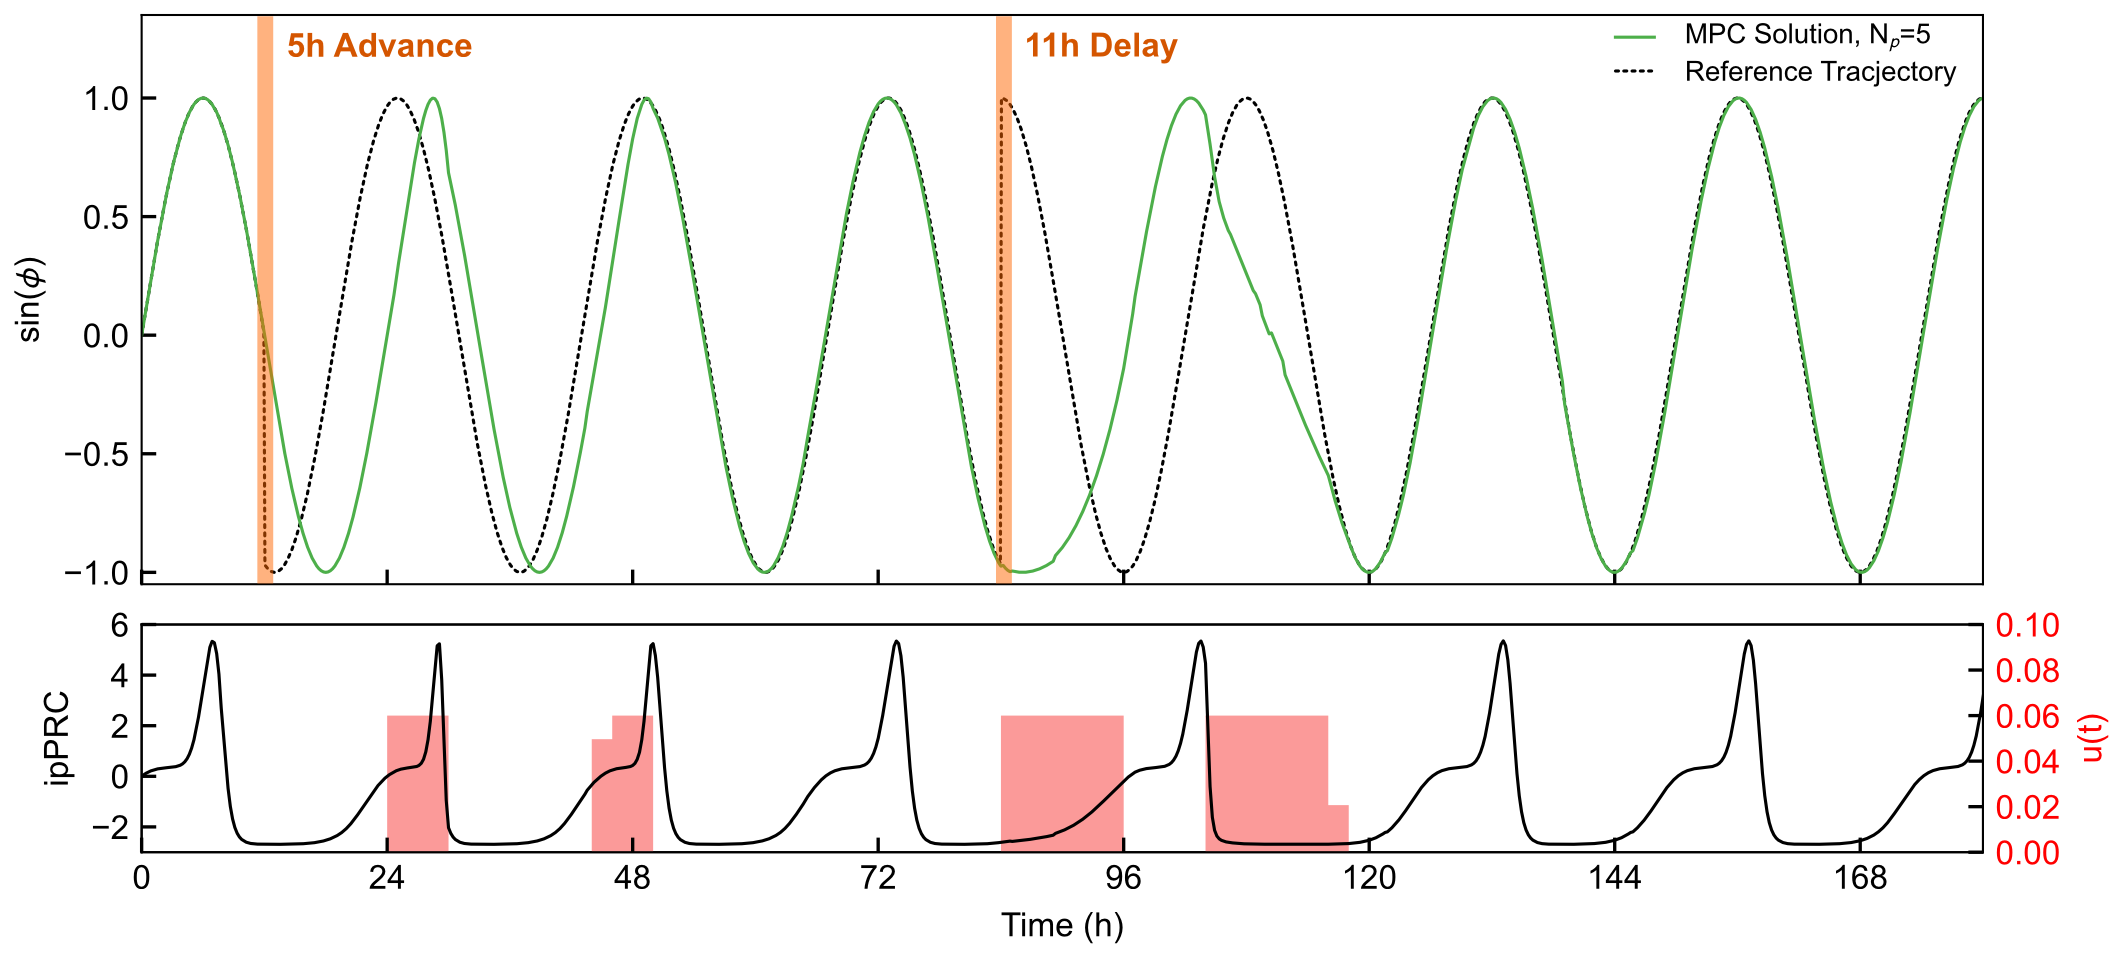
\includegraphics[width=\textwidth]{chap6/figures/figure_7.png}
\end{center}
      \caption{\label{fig:mpc_demo}
      Demonstration of MPC for phase resetting in response to jet lag. This scenario involves a 5h (0.417$\pi$ rad) phase advance followed by a 11h (0.917$\pi$ rad) phase delay, the equivalent of flying from Boston to London, then London to Honolulu three days later. (\textbf{A}) Phase of oscillator under MPC compared to reference phase (local time) for the jet lag problem. For this problem, $\tau=2$h and $N_p=5$. (\textbf{B}) Timing of control inputs and PRC throughout the simulation. In both cases, the reset is completely achieved in less than 48h, a drastic speedup in comparison to the untreated case or the light-input case \cite{Qiao2017}. For simplicity, no light input to the clock was assumed in this case, though it may be incorporated as an additional disturbance input to the phase model, or applied as part of multi-input control.
  }
\end{figure*}


\begin{figure*}[p]
    \begin{center}
    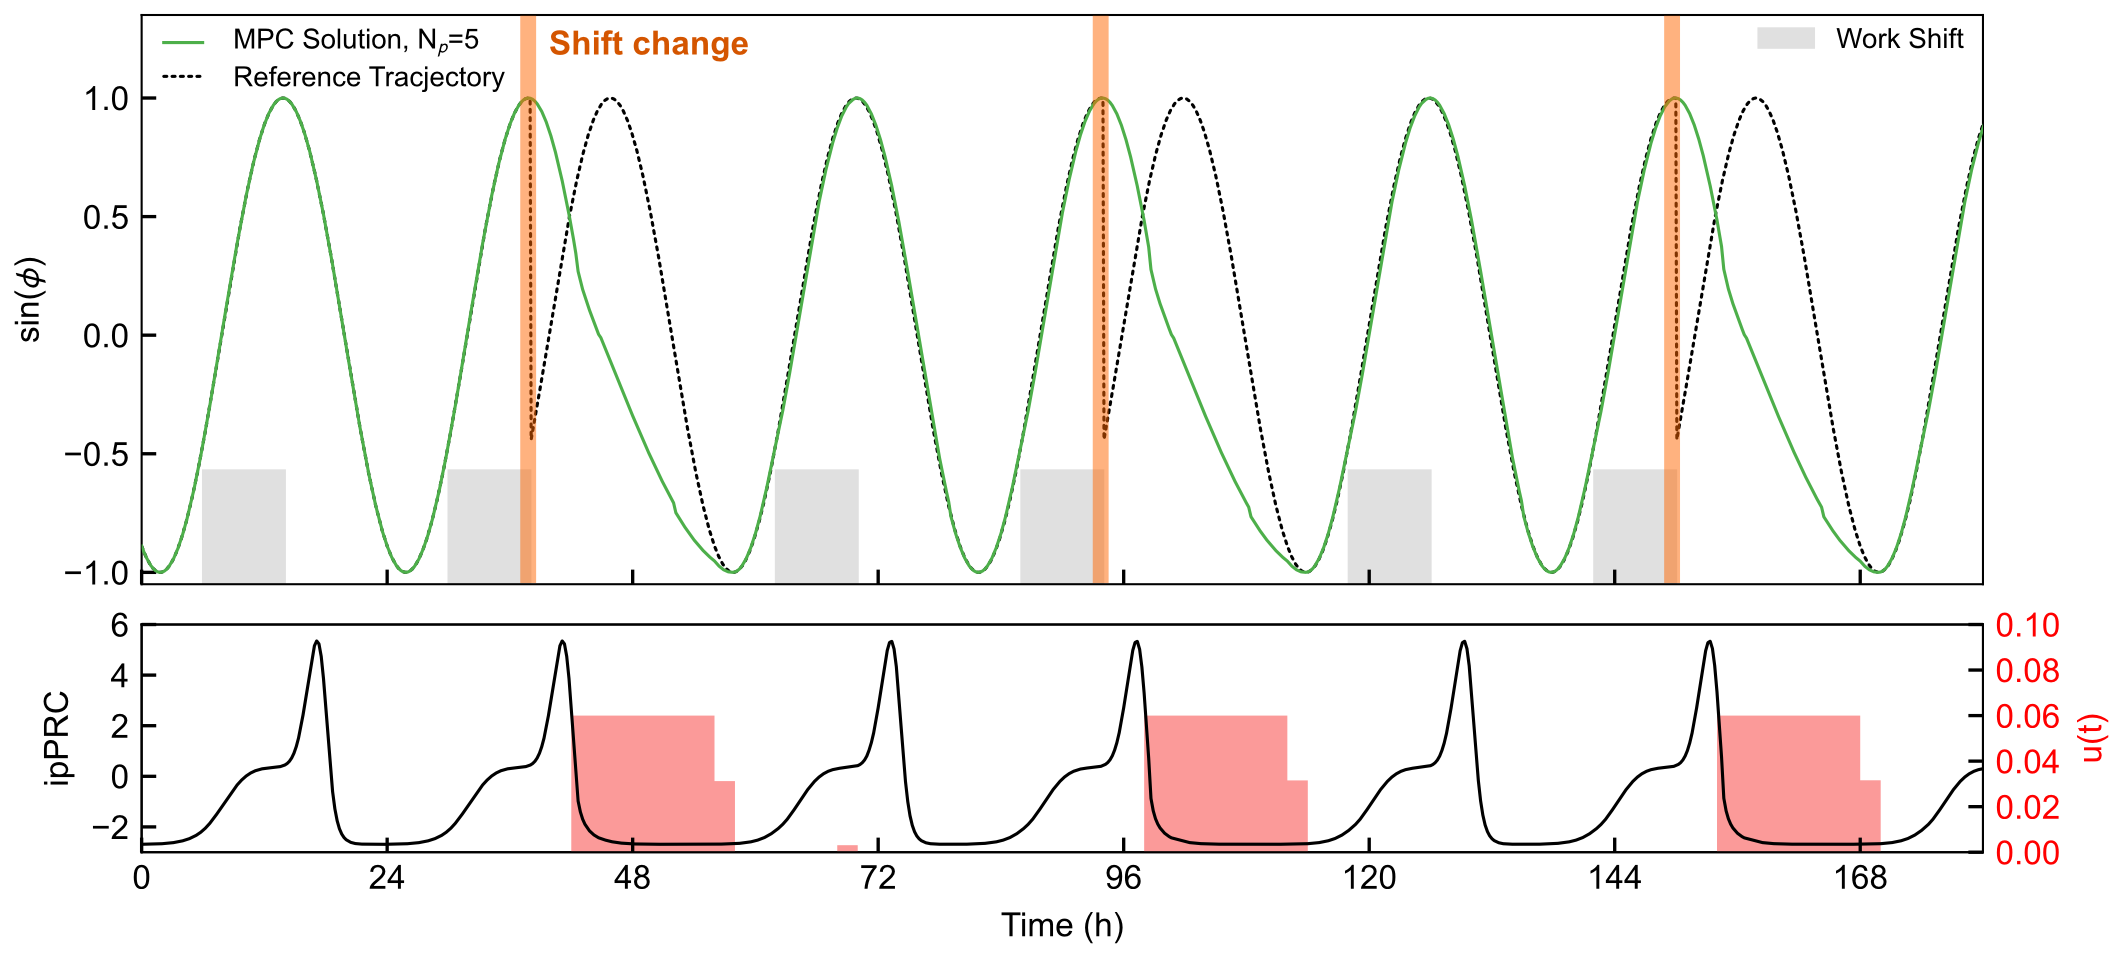
\includegraphics[width=\textwidth]{chap6/figures/figure_8.png}
\end{center}
      \caption{\label{fig:mpc_demo2}
      Demonstration of MPC for phase resetting in response to a weeklong rotating shift work schedule, described in \cite{Vetter2015}. This scenario involves 8h phase delays every two days when rotating from morning (06:00-14:00), to evening (14:00-22:00) to night (22:00-06:00) shifts, followed by days off. (\textbf{A}) Phase of oscillator under MPC compared to reference phase for the shift work problem. In this example, time corresponds to clock time, such that \textit{Per} expression in an individual entrained for morning work will occur near dusk. The reference phase was adjusted to the next rotating shift following the last work cycle of the prior rotating shift. For this problem, $\tau=2$h and $N_p=5$. (\textbf{B}) Timing of control inputs and PRC throughout the simulation. Because all shifts are achieved by delays, a slower sampling rate (longer duration between dosage changes) would have a similar efficacy. For simplicity, no light input to the clock was assumed in this case, though it may be incorporated as an additional disturbance input to the phase model, or applied as part of multi-input control.
  }
\end{figure*}

\clearpage
\section{Summary}
\label{sec:conc6}
This chapter presents tools for designing feedback control of circadian rhythms with explicit consideration for pharmaceutical inputs.
Importantly, this chapter provides a bound on the errors incurred by sampling time control of circadian oscillation, and may be applied to compare against the efficacy of a light-based approach; see, for example,~\cite{Qiao2017}.
Furthermore, it demonstrates the advantages provided by pharmacological actuation, as any phase reset is predicted to be achievable in under 60 h.
Uniquely, this work proposes a formulation of the nonlinear MPC based on the bounds derived from the optimal control problem.

Since drug discovery for the manipulation of circadian rhythms is ongoing, this chapter presents a perspective on which pharmaceuticals will enable control.
Specifically, an ideal circadian pharmaceutical will have (i) large-magnitude positive and negative ipPRC lobes, to enable bidirectional phase resetting, and (ii) rapid pharmacokinetics, to enable precise timing of its effect and minimal losses during ipPRC zero-crosses.
This is in contrast to traditional pharmaceutical approaches that select for a long drug half-life to ensure its effect is sustained.
Future studies should explicitly incorporate simple pharmacokinetic profiles, rather than piecewise-constant control.
However, achieving closed-form solutions or error bounds for these problems is challenging.

A remaining link in achieving closed-loop circadian control is the development of a noninvasive circadian phase sensor.
While phase may be assessed relatively simply from cellular bioluminescent reporters, noninvasive \textit{in vivo} phase inference in mammals is an open challenge.
Recent work in assessing phase from ambulatory monitoring has shown promise and reasonably accurate predictions \cite{Kolodyazhniy2012}, however, the propagation of measurement errors through such a control algorithm also remains an open question.
An ideal phase sensor would rely on simple data such as solely actigraphy, rather than additional biophysical sensors (e.g.\ skin temperature, salivary melatonin), and remains in development.
The abilities of phase inference methods and controller robustness will be of consequence for the implementation of any form of circadian feedback control mentioned herein.

Finally, this chapter has assumed the system under control to be a single oscillator and thus neglected the contributions of intercellular synchrony to circadian function.
A more detailed approach would involve controlling the multi-oscillator system with a multi-oscillator model, using formalisms developed in Chapter~1.
This problem could be approached through optimal control as in \cite{Li2013}.
Specifically, this would involve formulating the optimal control problem as a population of phase-only oscillators with identical PRCs but heterogeneous initial conditions, and possibly heterogeneous intrinsic frequencies.
Then, the minimum-power or time-optimal control problem can be solved with computational approaches, as analytic methods are intractable for large oscillator ensembles.
Alternately, this problem could be approached by simple augmentations to the MPC algorithm from this chapter.
In the following chapter, I demonstrate that the single-oscillator approach performs poorly under certain conditions where the oscillator is susceptible to desynchronization, and I present a simple approach to modify the nonlinear MPC of this chapter to correct for this issue.























